\documentclass[a4paper,12pt]{report}
\usepackage[utf8]{inputenc}
\usepackage[T1]{fontenc}
\usepackage[french]{babel}
\usepackage{microtype}  % pour éviter le coupage des mots
\usepackage{geometry}
\usepackage{caption}
\geometry{top=2cm, bottom=2cm, left=2cm, right=2cm}
\usepackage{setspace}
\usepackage{graphicx}
\usepackage[hidelinks]{hyperref}
\usepackage{url}
\usepackage{lipsum}
\usepackage{tocloft}
\renewcommand{\figurename}{Figure}
\renewcommand{\cftfigpresnum}{Figure\ } % Texte à afficher avant le numéro de la figure
\setlength{\cftfignumwidth}{3cm}       % Largeur de la boîte pour les numéros de figures

\renewcommand{\thesection}{\arabic{section}}
\usepackage{chngcntr} % Package pour la gestion des compteurs
\setcounter{tocdepth}{3} %inclure subsubsection dans la table des matieres
\renewcommand\thesubsubsection{\thesubsection.\arabic{subsubsection}}
\usepackage{enumitem} % Pour ajuster les marges


\usepackage{csquotes}
\usepackage[backend=biber,style=numeric,url=false]{biblatex}
\addbibresource{references.bib}

\begin{document}

% Page de garde
\begin{titlepage}
  \begin{center}
  \centering
  
  \begin{minipage}{0.45\textwidth}
    \raggedright
    
\includegraphics[width=\textwidth]{images/logo/logo_univ.png}
  \end{minipage}
  \hfill
  \begin{minipage}{0.25\textwidth}
      \raggedleft
      
\includegraphics[width=\textwidth]{images/logo/logo_cnieg.png}
  \end{minipage}

  \vspace{3cm}

  {\scshape\LARGE Rapport de stage \par}
  \vspace{1cm}
  \rule{\textwidth}{0.8pt} \\ 
  \vspace{0,2cm}

  \textbf {Réalisation d’une application web de notation de formation pour les agents de la CNIEG avec Angular / Spring Boot }

  \vspace{0,1cm}
  \rule{\textwidth}{0.8pt} \\ %line Horizontale
  
  \vspace{1cm}
  
  {\Large 15 mars 2024 - 7 juin 2024 \par}
  \vfill
\end{center}

\noindent
\hspace{2cm}\textbf{Réaliser par } \hspace{1cm} Amina BOUDJEDIR

\vspace{1.5cm}

\noindent
\hspace{2cm}\textbf{Encadrants} \\
\begin{tabbing}
  \hspace{4cm} Entreprise \hspace{2,9cm} Clément SIROU \\
  \hspace{4cm} Université de Nantes \hspace{1cm} Amal TIAB
\end{tabbing}
\vfill

\begin{center}
    Année universitaire 2023 - 2024
\end{center}

  
\end{titlepage}

% Remerciment
\chapter*{Remerciements}
Au moment où s'achèvent la réalisation du projet et la rédaction de ce rapport, 
il m'est agréable de me retourner avec gratitude vers ceux qui  m'ont apporté leur 
indispensable assistance dans cette aventure.
\medskip

Tout d'abord, je tiens à travers ces quelques lignes, adresser ma profonde gratitude 
et mes sincières remerciements à mon tuteur, M. Clément SIROU pour tout son soutien et aide 
qu'il m'a apporté durant toute la période de mon stage, ainsi que pour ses précieux 
conseils et ses encouragements aux moments de doute.
\medskip

Enfin, à mes proches, merci pour votre présence, vos encouragements furent sans nul doute, 
ma plus grande source de motivation.



% Sommaire
\tableofcontents
\newpage

\chapter*{Introduction}
\addcontentsline{toc}{chapter}{Introduction}
Du 15 mars au 7 juin j’ai eu l'opportunité de rejoindre la CNIEG en tant que développeuse full stack sous 
la gouvernance de M Clément SIROU, un développeur au sein de cette entreprise. 
Naturellemnt, attiré par le milieu de  la programmation j'ai rappidement décidé d'orienté mes recherches 
de stage vers ce domaine.\medskip

Le but de ce stage est de parvenir à réaliser et à développer un produit minimun viable en utilisant 
des technologies modernes.\medskip

Ce rapport présente les différentes tâches et missions que mon tuteur m'a confié, elles se dévisent en 3 parties : 
\medskip

Avant tout une présentation de l'entreprise, de l'équipe de travail, leurs méthologie de travail et du cadre général de ce projet.\medskip

Ensuite je me focalise sur le cahier des charges et les demandes du client.\medskip

Et enfin la troisième partie présente tout d'abord les technologies utilisées et l'architechture du 
logiciel avec ses deux aspect front et back. Elle détaille également les besoins fonctionnels et non fonctionnels 
et aborde l'analyse de ces besoins en se basant sur le langage de modélisation UML. 

\medskip
   
    \section{CNIEG}
    La Caisse Nationale des Industries Electriques et Gazières (CNIEG) a été créée le 1er janvier 2005 par la loi du 9 août 2004 en tant qu’organisme de sécurité sociale de droit privée, doté d’une personnalité morale. Il existe un seul site qui se trouve à Nantes, 20 rue des Français libres.
	\medskip

    La CNIEG est une caisse de retraite chargée de la gestion du régime spécial d’assurance vieillesse, invalidité, décès, accidents du travail et maladies professionnelles des industries électriques et gazières (IEG).
	L’entreprise ne fonctionne pas avec une structure hiérarchique classique. En effet la CNIEG a pour but d’être une entreprise « responsabilisante ».
    \medskip

	L’entreprise est divisée en départements :
    \medskip
    \begin{itemize}[leftmargin=2cm]
        \item Direction
        \item Département audit comptable finance (DACF).
        \item Département secrétariat général.
        \item Département gestion et relation clientèle (DGRC).
        \item Département système d’information (DSI).
    \end{itemize}
	\medskip

	Chaque département est composé de plusieurs pôles.

    
  % ...

    \section{Équipes de travail}
    Mon stage se déroule au sein du département système d’information dans l’équipe Pégase. Ce département est constitué de plusieurs pôles :
    \medskip

	Pôle pilotage SI : expérimentées, pragmatique et pédagogiques pour réussir les projets management de projet.
	\medskip

    Pôle GPSI
	\medskip

    Pôle conduite : contrôle et analyse, planifications, suivi d’évolution, Bilan compte rendu remonté d’incident.
	\medskip

    Pôle exploitation : Gestion des demandes et incidents, Mise en production, Réseau Téléphonie Infrastructure, gestion des contrats d’infogérance, gestion du parc informatique, traitement et flux.
	\medskip

    Pôle A2iD : Architecture Infrastructure Intégration Déploiement.
	\medskip

    Pôle IED : Ingénieur études et Développement.
	\medskip

    Pôle ISI : Ingénieur Système d’Information.
	\medskip

    Co-DSI : gestion des richesses humaines de DSI.
    \medskip

    Domaine de travail :  gestion et paiement, carrière et financement, interactions clients.
    \medskip

    Equipes de réalisations : Belem, Albatros, Glenan, Capri, Phoenix, Pégase.
    \medskip

	Dans ce département il y a plusieurs équipes chacune composée de Business analyst (BA), de développeur (DEV), dun product owner (PO) et d'un scrum master (SM) qui travaillent en collaboration.




    \section{Méthodologie de travail} 
    La CNIEG adopte une approche agile dans la gestion de ses projets de développement logiciels. Cette approche vise à favoriser la flexibilité, la réactivité et la livraison continue de valeur ajoutée, dans ce qui suis une description de cette approche au sein de l'entreprise :  
    \medskip
    \begin{enumerate}
        \item Planifiaction\\Sélection des fonctionnalités : L’équipe de développement avec les parties prenantes, identifie les fonctionnalités à développer pour répondre aux besoins de l'entreprise et des utilisateurs.\\Élaboration du backlog : liste prioritaire de fonctionnalités qu’un produit doit contenir, sous forme de 'user story' ou de tâches.
        \medskip
        \item Itérations\\Les développements sont organisés en sprints d'une durée de 3 semaines dans laquelle l’équipe s’engage à livrer un ensemble défini de fonctionnalités.\\
        Au début de chaque sprint, l’équipe sélectionne un ensemble de user story à réaliser, en fonction de leur priorité et de la capacité de l’équipe.\\
        Chaque jour l’équipe se rassemble pour une réunion quotidienne(mêlée) afin de partager l’avancement, les obstacles éventuels et les plans de la journée.
        \medskip

        \item Développement\\Les membres de l'équipe collaborent étroitement tout au long du processus de développement, en partageant leurs connaissances et en résolvant les problèmes ensemble.
        \medskip

        \item Revue et rétrospective\\Une fois le sprint terminé, l’équipe présente les fonctionnalités développées aux parties prenantes pour obtenir leur feedback et valider les livrables.\\L’équipe se réunit pour réfléchir sur le sprint écoulé, identifier ce qui a bien fonctionné et ce qui peut être amélioré, afin d’ajuster et d’optimiser le processus pour les sprints suivants.
        \medskip   
    \end{enumerate}
        \subsection{Processus de développement} 
        Dans leurs processus de développement logiciel, Git est utilisé comme plateforme de gestion de code source. Les développeurs travaillent sur leurs branches, et lorsqu’ils finalisent leur code, ils le poussent vers Gitlab.
        \medskip

	    Ensuite, Jenkins entre en jeu. Il surveille en permanence les modifications sur Gitlab. Dès qu’un développeur pousse du code sur une branche, Jenkins lance un build (compilation du code, tests automatisés) de cette branche. Si le build est KO il envoie un message à l’auteur du commit, sinon si le build est OK alors les fichiers 'pom' sont exécutés et des packages 'jar' ou 'war' seront générés. Une fois l’image construite générée, elle sera stockée dans Nexus qui est un gestionnaire de paquet.
        \medskip

	    Enfin, Kubernetes orchestre le déploiement des applications. Un exemple de son utilisation au sein de l’entreprise : En fin de mois le back paie qui est très sollicité va faire appel à beaucoup de service pour récupérer les informations. L’application a une instance (Pod) qui tourne et qui se fait 'bombarder' alors Kubernetes lance une autre instance pour répondre à la forte demande qui est automatique. Un des avantages de son utilisation : pas d’impact sur le SI, stable. 
        \medskip

        En revanche, les équipes envisagent une transition vers Gitlab CI pour améliorer leurs processus d'intégration et de déploiement continu.
        Gitlab CI simplifie et permet d'optimiser le processus de développement en intégrant de manière plus fluide l'intégration et le déploiement continu.\medskip

        Nous allons adopter cette approche dans notre projet, ce qui nous permettra de bénificier d'une configuration et intégration plus simple.
        
  % ...

\chapter*{Contexte du projet}
\addcontentsline{toc}{chapter}{Contexte du projet}

L’objectif du projet est de créer une application web qui permet aux agents de l’entreprise de noter les formations qu’ils ont suivi.
\medskip

La CNIEG souhaite encourager les agents à être acteurs de leur parcours professionnel et à identifier les formations qui répondent le mieux à leurs besoins. L'objectif est de créer un outil collaboratif qui permet aux agents de partager leurs expériences et leurs avis sur les formations suivies. 
Nous avons pris contact avec le service Ressources Humaines pour définir les besoins fonctionnels et les caractéristiques de l’application.
\medskip

Spécification des besoins fonctionnels :
\begin{enumerate}[leftmargin=2cm]
    \item \textbf{Donner son avis :} les agents peuvent donner leurs avis sur les formations qu'ils ont suivies, en évaluant différents aspects de la formation (organisation, durée, contenu, etc.).
    \item \textbf{Consulter les avis :} les agents peuvent consulter les avis des autres collègues sur les formations suivies, pour s'inspirer et vérifier la qualité de la formation dispensée.
\end{enumerate}
\medskip

Caractéristiques :
\medskip
\begin{itemize}[leftmargin=2cm]
    \item L'application est accessible à tous les agents de la CNIEG.
    \item L'application est complémentaire de l'évaluation à froid adressée par le pôle RH 3 à 4 mois après les formations.
    \item Le lien de l'application est envoyé par mail après chaque formation réalisée, et est également disponible sur le SharePoint - espace salarié.
\end{itemize}
\medskip

Items d'évaluation :
\medskip
\begin{itemize}[leftmargin=2cm]
    \item Organisation de la formation (convocation, plan d'accès, lien de connexion si formation à distace, locaux...)
    \item Durée de la formation.
    \item Avez-vous appris des choses nouvelles ?
    \item La formation a-t-elle répondu à vos attentes ?
    \item Etc. (items à définir)
\end{itemize}
\medskip

Système d'évaluation :
\medskip
\begin{itemize}[leftmargin=2cm]
    \item Chaque item d'évaluation a un nombre d'étoiles associé (entre 1 et 5).
    \item Chaque item d'évaluation a une zone de commentaire libre.
\end{itemize}
\chapter*{Travail réalisé}
\addcontentsline{toc}{chapter}{Travail réalisé}
\setcounter{section}{0} % Réinitialisation du compteur de section

\section{Technologies utilisées}

\begin{center}
    \begin{minipage}{\textwidth}
        \begin{minipage}{0.2\textwidth}
            \centering
            
\includegraphics[width=1\textwidth]{images/logo/angular.jpeg}
        \end{minipage}\hfill
        \begin{minipage}{0.75\textwidth}
            \textbf{Angular} est un framework de développement frontend avec une structure modulaire. Permet de créer des applications web de type SPA (Single page application) dynamiques et robustes.
        \end{minipage}
    \end{minipage}

    \vspace{2em} % Espace entre les figures

    \begin{minipage}{\textwidth}
        \begin{minipage}{0.2\textwidth}
            \centering
            
\includegraphics[width=0.5\textwidth]{images/logo/springBoot.png}
        \end{minipage}\hfill
        \begin{minipage}{0.75\textwidth}
            \textbf{Spring Boot 3} est un framework Java open source, un framework de développement backend, pour simplifier et accélérer le développement d'application Java.
        \end{minipage}
    \end{minipage}


    \vspace{2em} % Espace entre les figures
    
    \begin{minipage}{\textwidth}
        \begin{minipage}{0.2\textwidth}
            \centering
            
\includegraphics[width=0.4\textwidth]{images/logo/typeScript.png}
        \end{minipage}\hfill
        \begin{minipage}{0.75\textwidth}
            \textbf{TypeScript} est un sur-ensemble du langage JavaScript dont j'ai eu l'occasion de découvrir lors de mon parcours universitaire, ajoutant de nouvelles fonctionnalités et syntaxes.
        \end{minipage}
    \end{minipage}

    \vspace{2em} % Espace entre les figures
    
    \begin{minipage}{\textwidth}
        \begin{minipage}{0.2\textwidth}
            \centering
            
\includegraphics[width=0.5\textwidth]{images/logo/postgres.svg.png}
        \end{minipage}\hfill
        \begin{minipage}{0.75\textwidth}
            \textbf{PostgreSQL} est un système de gestion de base de données relationnelles. On a choisi cette base car l'entreprise a privilégié de migrer toutes ses applications sur PostgreSQL, car les licences Oracle deviennent plus chères.
        \end{minipage}
    \end{minipage}

    \vspace{2em} % Espace entre les figures
    
    \begin{minipage}{\textwidth}
        \begin{minipage}{0.2\textwidth}
            \centering
            
\includegraphics[width=0.5\textwidth]{images/logo/ittelij.jpg}
        \end{minipage}\hfill
        \begin{minipage}{0.75\textwidth}
            \textbf{IntelliJ IDEA 2024.1} comme environnement de développement de l'application.
        \end{minipage}
    \end{minipage}

    \vspace{2em} % Espace entre les figures
    
    \begin{minipage}{\textwidth}
        \begin{minipage}{0.2\textwidth}
            \centering
            
\includegraphics[width=0.35\textwidth]{images/logo/flyway.png}
        \end{minipage}\hfill
        \begin{minipage}{0.75\textwidth}
            \textbf{Flyway} est un outil de migration de base de données qui permet de gérer et d’automatiser les versions des schémas de base de données de manière cohérente.
        \end{minipage}
    \end{minipage}

    \vspace{2em} % Espace entre les figures
    
    \begin{minipage}{\textwidth}
        \begin{minipage}{0.2\textwidth}
            \centering
            
\includegraphics[width=0.5\textwidth]{images/logo/maven.png}
        \end{minipage}\hfill
        \begin{minipage}{0.75\textwidth}
            \textbf{Maven} est un outil de gestion de la construction de logiciels. Il aide à compiler et tester un logiciels, mais aussi à le distribuer et à le rendre simple à comprendre par d'autres développeurs.
        \end{minipage}
    \end{minipage}
\end{center}

\newpage

\section{Architecture}
Dans le cadre de mon stage, j'ai eu l'occasion d'explorer la dynamique entre les différentes technologies utilisées. L'architecture du projet se schématise de la façon suivante :
\medskip

\begin{figure}[h!]
    \centering
    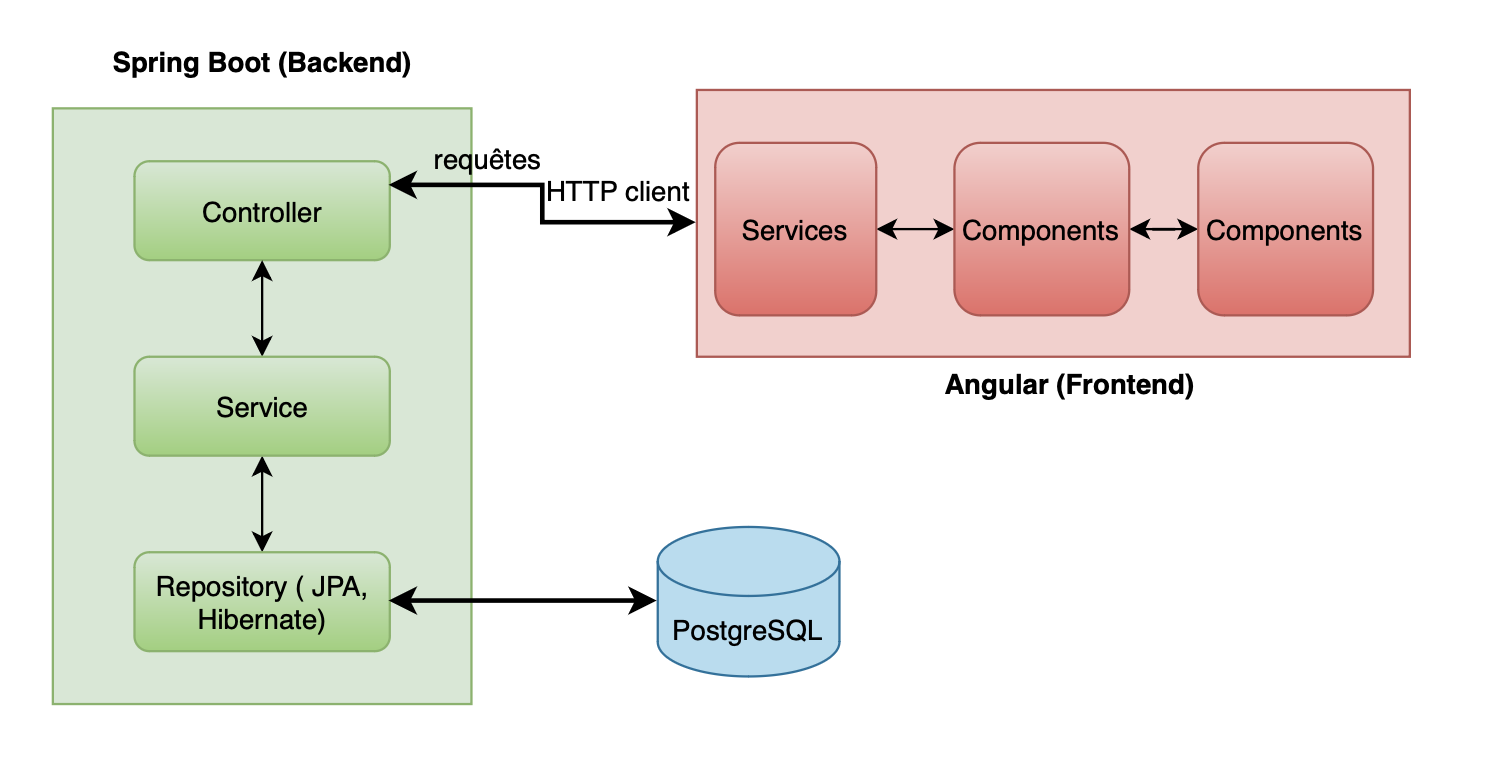
\includegraphics[width=0.8\textwidth]{images/diagramme/archi.png}
    \caption{Architecture de l'application}
\end{figure}
\medskip

Cette représentation illustre la manière dont les différentes technologies interagissent entre elles. Les éléments qui participent à l'interaction entre l'utilisateur, l'application et la base de données sont le 'Controller', le 'Service' et le 'Repository'. Chacun ayant un rôle spécifique :
\medskip

Controller : gère les interactions entre l'utilisateur et l'application, agissant comme un pont entre l'utilisateur et l'application. Il reçoit et traite les requêtes de l'utilisateur et dirige les actions appropriées vers les services correspondants.
\medskip

Service : implémente les traitements nécessaires pour répondre aux demandes de l'utilisateur. il interagit avec les 'Repository' pour accéder aux données. 
\medskip

Repository : gère l'interaction avec la base de données, il utilise JPA, un framework ORM, pour mettre en pratique le patrons de conception DAO pour exécuter des requêtes SQL sans avoir besoin de les écrire. Cette approche facilite la communication avec la source de données.
\medskip

\subsection{Mise en place}
Concernant la mise en place du projet, nous avons suivi les étapes suivantes :
\medskip

\textbf{Mise en place de la stack et configuration de l'environnement de développement} : Nous avons débuté par la création d'un dépot Git pour la gestion collaborative du code source, suivi de la configuration de la structure du projet et de son environnement à l'aide de Docker. Docker nous permet de créer des images systèmes adaptées à nos besoins, tandis que NGINX a été utilisé comme serveur pour exposer les services de notre application Angular.
\medskip

Une fois l'image construite elle sera hébergée, déployée sur Kubernetes, qui est un orchestrateur qui permet de gérer les images dockers, permet de déployer des services. Kubernetes va lancer l'image et exécuter le fichier 'entrypoint.sh' qui démarre notre service Angular avec la commande  `ng serve`.
\medskip

\textbf{Création des squellettes backend et frontend :} Nous avons utilisé les outils Spring Initializr et Angular CLI pour générer les squellettes de nos projets backend et frontend respectivement. En personnalisant ensuite les configurations de base pour le projet Anguler. Cette approche nous a permis de démarrer rapidement le développement.
\medskip

    \subsection{Partie frontend}
    Le développement a débuté par la mise en place de l'interface utilisateur qui repose sur le framework Angular. Les composants ont été créés progressivement en fonction des exigences fonctionnels de l'application. Cela a permis de prendre en mains le framework Angular et de comprendre comment il fonctionnait.
    \medskip

    L'application est divisée en plusieurs composants qui intéragissent avec les services, dont la figure ci-dessous illustre les différents composants :
    \medskip

    \begin{figure}[h!]
        \centering
        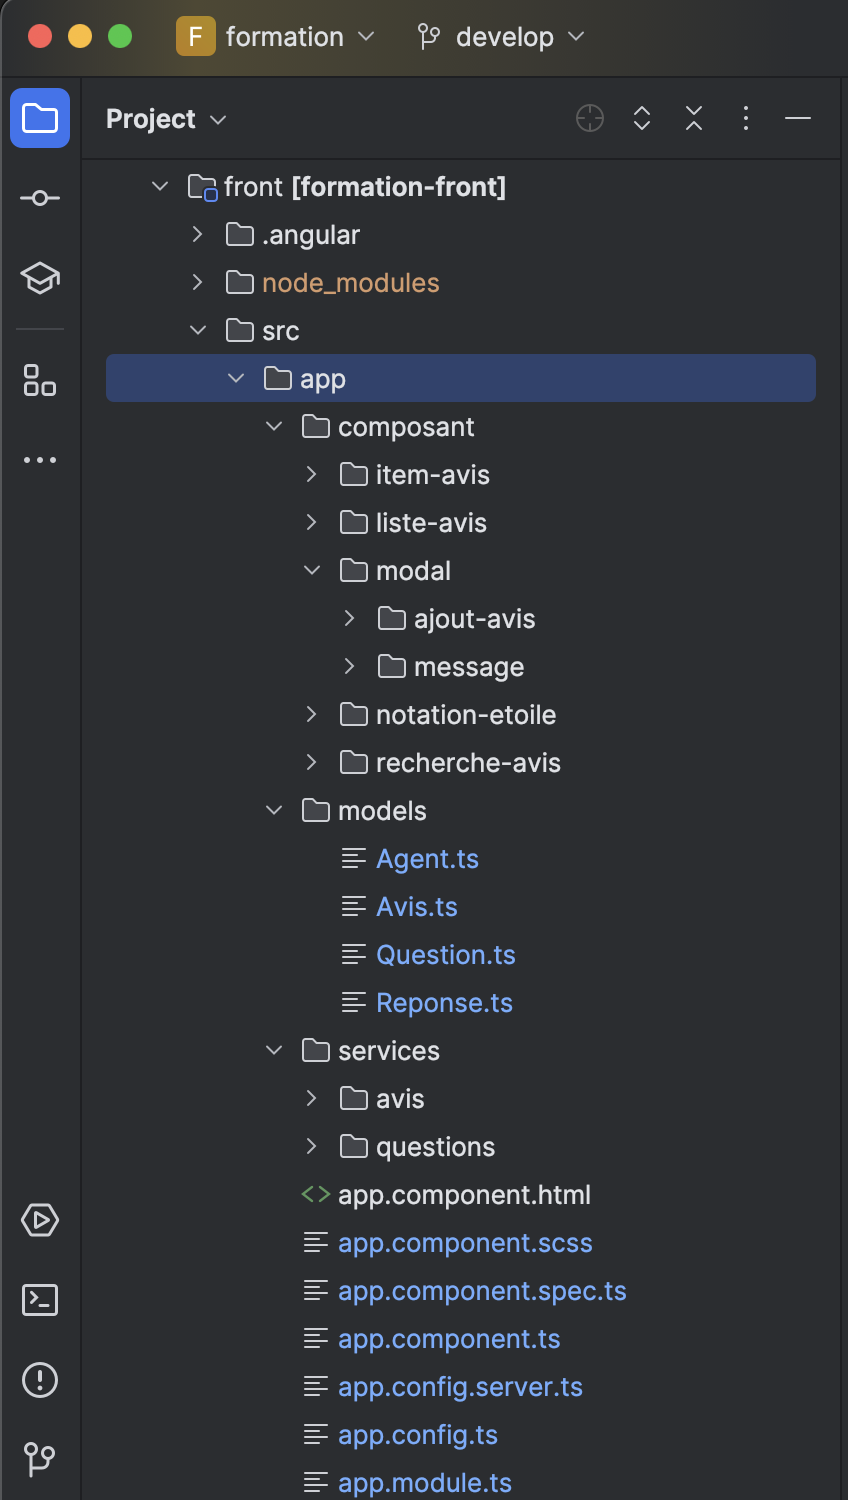
\includegraphics[width=0.5\textwidth]{images/code/composant.png}
        \caption{Les différents composants de l'application}
    \end{figure}
    \medskip

    Les différents composants sont les suivants :
    \medskip

    \begin{itemize}
        \item Le composant ajout-avis, qui représente une fenêtre modale permettant l'affichage du formulaire de création ou affichage de l'avis.
        \item Le composant liste-avis, qui représente la page web principale pour l'affichage de la liste des avis.
        \item Le composant item-avis, qui représente chaque item d'un avis, chacun composé d'une note et d'un commentaire.
        \item Le composant notation-etoile, qui représente un système de notation par étoiles.
        \item Le composant recherche-avis, qui représente le composant de la barre de recherche d'un avis.
        \item Le composant message, qui permet la gestion des notifications.
    \end{itemize}
    \vspace{0.5cm}

    Deux services sont utlisés dans l'application pour gérer les opérations communes entre les composants.  Ces services ont le rôle de pont entre les composants et les appels HTTP à l'API backend de l'application.    
    \medskip

    Le service avis a les fonctionnalités suivantes :
    \medskip
    
    \begin{itemize}
        \item Récuperer tous les avis : cette fonctionnalité permet de récuperer les avis à partir de l'API backend en envoyant une requête HTTP GET.
        \item Ajouter un avis : cette fonctionnalité permet d'ajouter un avis en envoyant une requête HTTP POST à l'API backend pour ajouter l'avis dans la base de données.
        \item Chercher un avis : cette fonctionnalité permet de chercher un avis à partir d'une information spécifique en envoyant une requête HTTP GET à l'API backend.
    \end{itemize}
    \medskip

    Le service question a la fonctionnalité suivante :\medskip
    \begin{itemize}
        \item Récuperer toutes les questions : cette fonctionnalité permet de récuperer les questions du formulaire de notation à partir de l'API backend en envoyant une requêtes HTTP GET.
    \end{itemize}\medskip
    
    \subsection{Partie backend}
    Avant de commencer l'implémentation de la partie back, il est crucial de définir clairement notre modèle de données et les interactions utilisateurs via des diagrammes UML. Ces représentations graphiques nous permettent de visualiser et de structurer la solution objet de manière claire et précise. 
    \medskip
    \subsubsection{2.2.1\hspace{2em}Diagramme des cas d'utilisation}
        Ce diagramme permettra de décrire le dialogue entre les acteurs dans notre cas les agents et leurs tâches à accomplir sans ambiguïté. Il donne une vision globale du comportement fonctionnel.
        \medskip

        \begin{figure}[h!]
            \centering
            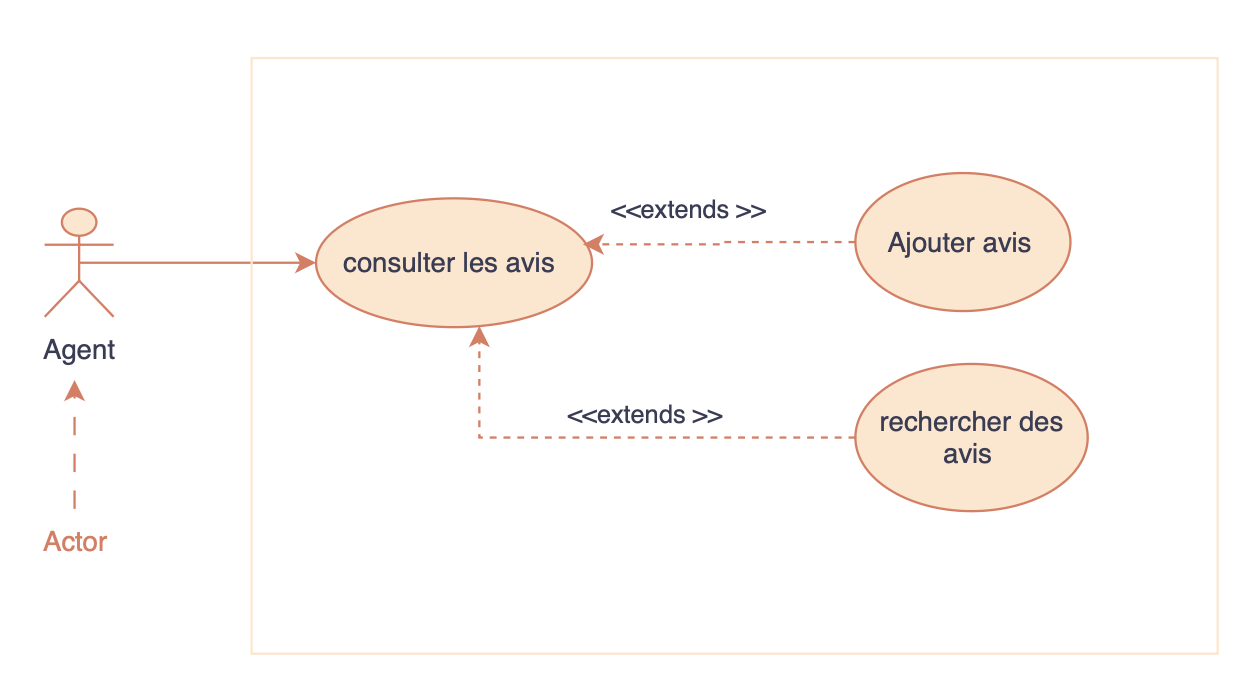
\includegraphics[width=0.8\textwidth]{images/diagramme/casUtilisation1.png}
            \caption{Diagramme de cas d'utilisation}
        \end{figure}
        \vspace{7cm}

        \subsubsection{2.2.2\hspace{2em}Diagramme d'activité}
        Le diagramme d'activité suivant, permet d'illustrer les différents choix que l'utilisateur pourra faire. Ce diagramme nous montre les actions des différents boutons.
        \medskip

        \begin{figure}[h!]
            \centering
            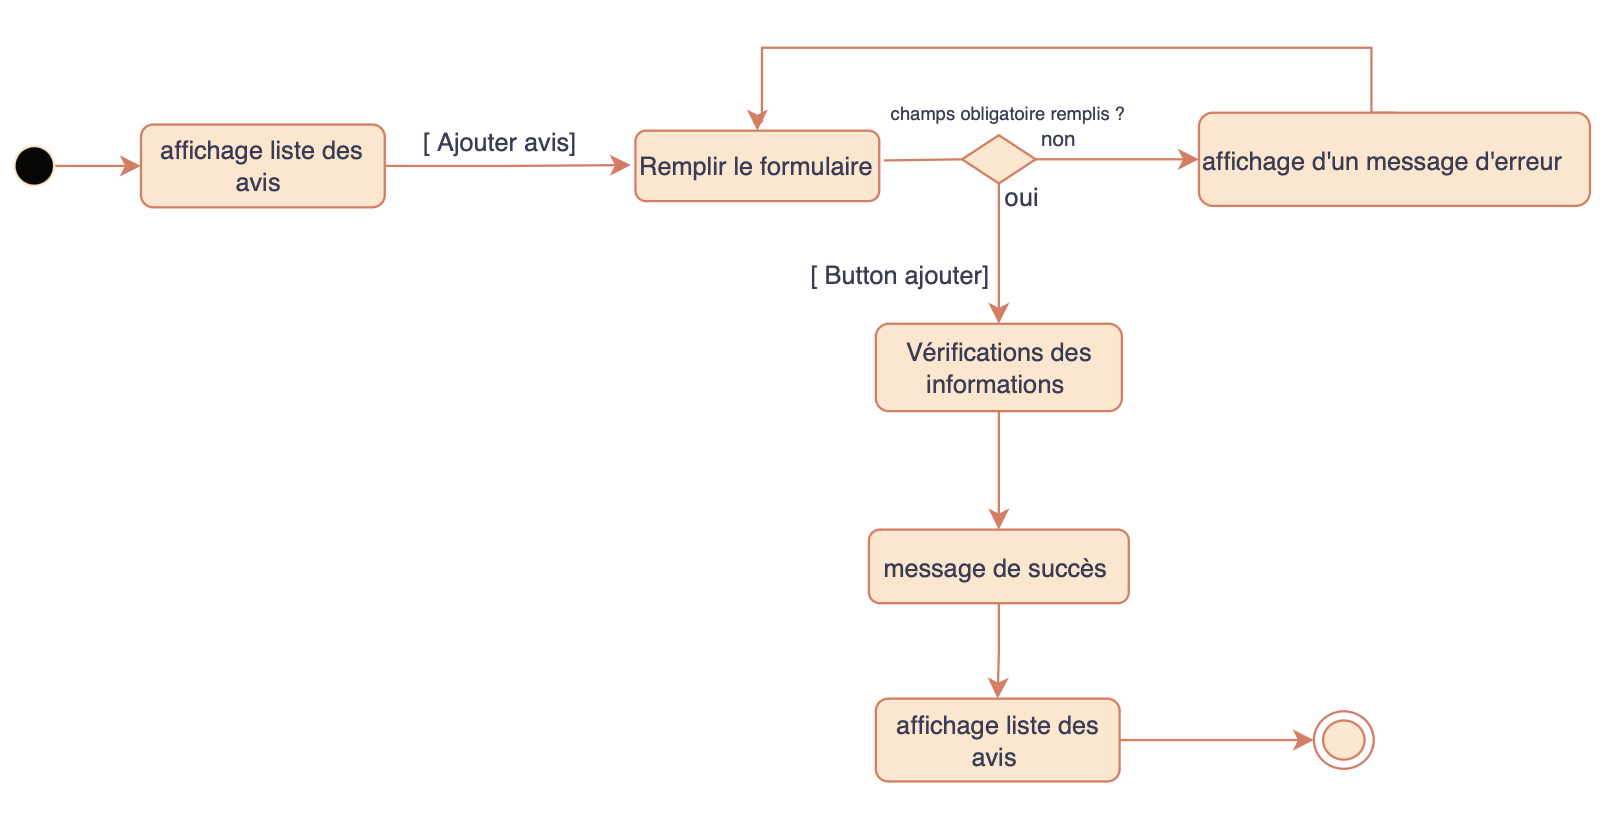
\includegraphics[width=0.9\textwidth]{images/diagramme/activite.png}
            \caption{Diagramme d'activité du cas d'utilisation ajouter avis}
        \end{figure}
        \medskip

        \subsubsection{2.2.3\hspace{2em}Diagramme de classe}
        Après réflexion avec mon tuteur sur le modèle de données le plus adapté pour représenter les données, nous sommes arrivés au diagramme de classe suivant :
        \vspace{3cm}

        \begin{figure}[h!]
            \centering
            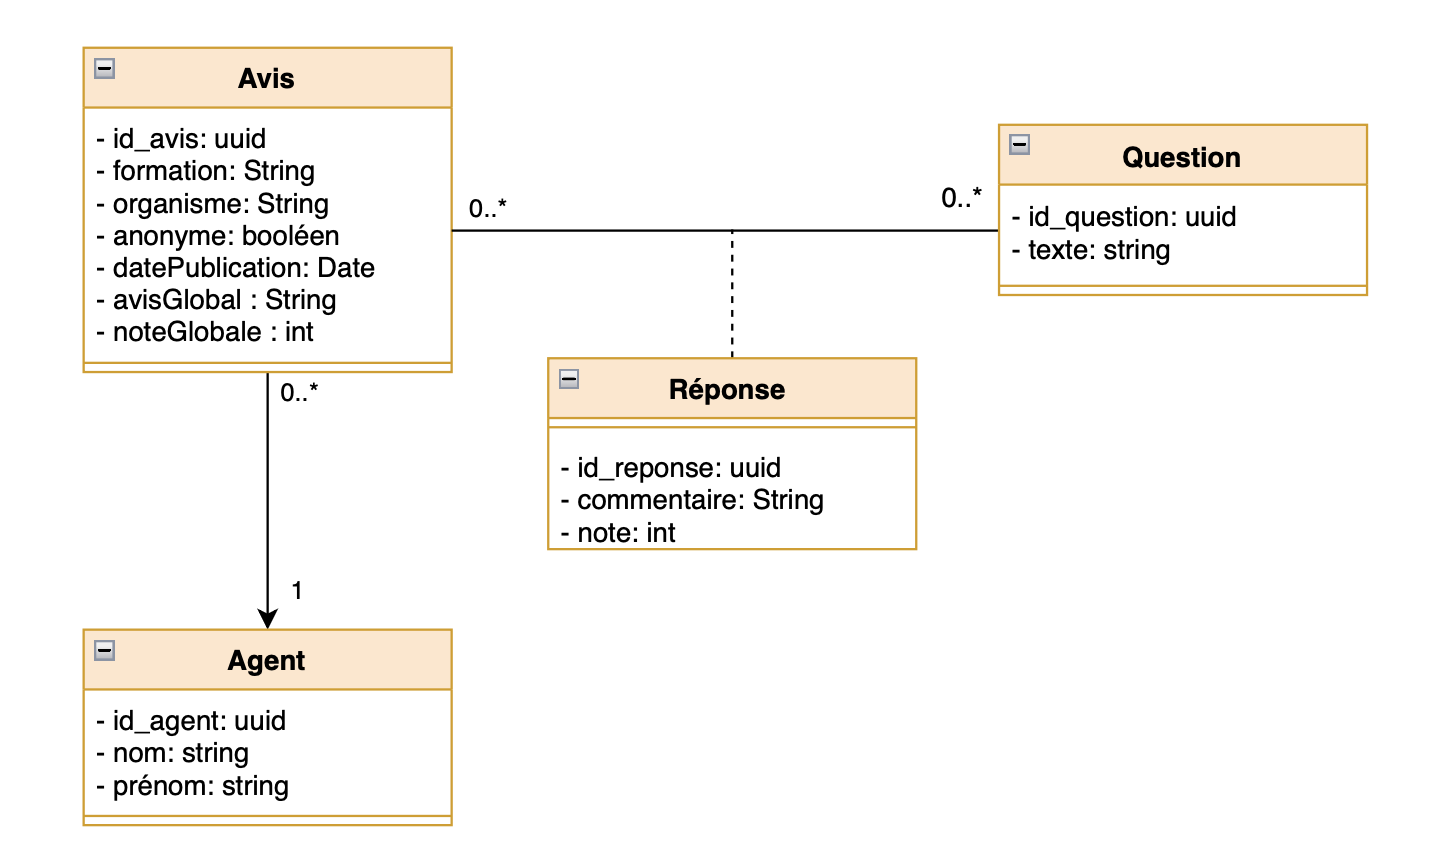
\includegraphics[width=0.9\textwidth]{images/diagramme/cllasse.png}
            \caption{Diagramme de classe UML}
        \end{figure}
        \medskip
    
        \subsubsection{2.2.4\hspace{2em}Choix techniques et implémentation}
        Dans un premier temps, nous avons utilisé une base de données H2 avec Spring Boot. 
        H2 est une base de données rapide et légère qui offre la possibilité d'une persistance 
        dans un fichier.\medskip
        
        Lors du développement du service backend, une bonne pratique pour travailler avec les 
        bases de données est de ne pas utiliser la génération et la mise à jour automatique du 
        schéma avec Hibernate/JPA, mais plutôt utiliser Flyway, qui est un outil de migration 
        de base de données qui met à jour la base de données de manière cohérente et contrôlée.\vspace{0.5cm}

        Aprés avoir défini et visualisé notre modèle de données à l'aide des diagrammes UML, 
        nous avons commencé par créer les classes entités définies dans le diagramme de classes.
        \vspace{11cm}

        \begin{figure}[h!]
            \centering
            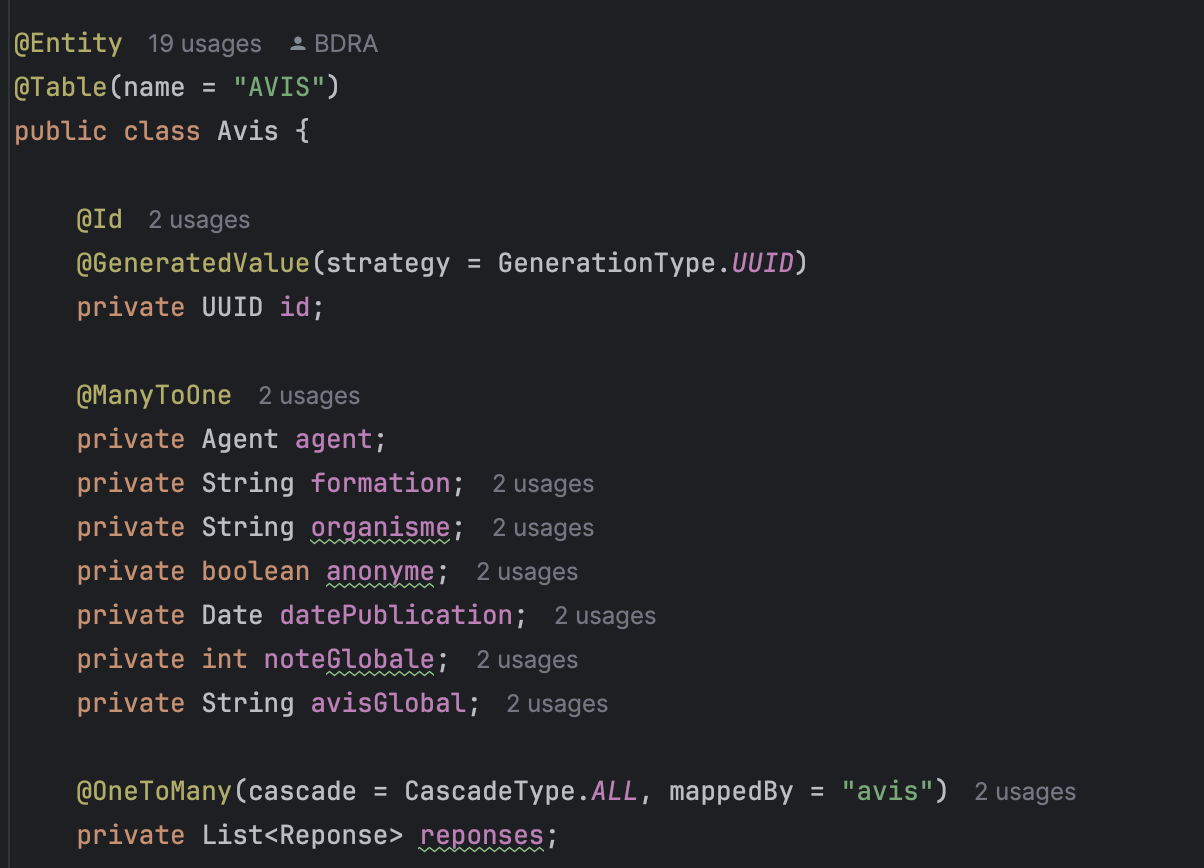
\includegraphics[width=0.8\textwidth]{images/code/avisEntity.png}
            \caption{Exemple de classe model de l'application}
        \end{figure}\medskip

        Les différentes classes Java comportent plusieurs notations :
        \medskip
        
        \textbf{@Entity}: permet à Hibernate/JPA de les considérer comme des ORM qui transfère les données entre l'application et la base de données.
        \medskip

        \textbf{@Table}: permet de mapper l'entité en table physique dans la base de données.
        \medskip

        \textbf{@Id}: permet d'identifier un attribut de la classe comme clé primaire de la table.
        \medskip

        \textbf{@GeneratedValue(strategy = GenerationType.UUID)}: est utilisée pour spécifier la stratégie de génération de clé primaire. L'attribut 'strategy' détermine comment la clé primaire est générée, dans ce cas elle est sous forme de UUID.\medskip

        \textbf{@Column}: permet de mapper un attribut de la classe à une colonne de la table.
        \medskip

        \textbf{@ManyToOne, @OneToMany}: permet de gérer les associations (*, 1) et (1, *) entre deux entités.
        \vspace{1cm}

        Pour transfèrer nos données entre les différentes couches de notre application de manière optimisée, nous avons adopté l'utilisation des classes DTO (Data Transfer Object).
        Les classes DTO sont des objets simples utilisés pour tranférer uniquement les données nécessaires.\medskip

        \begin{figure}[h!]
            \centering
            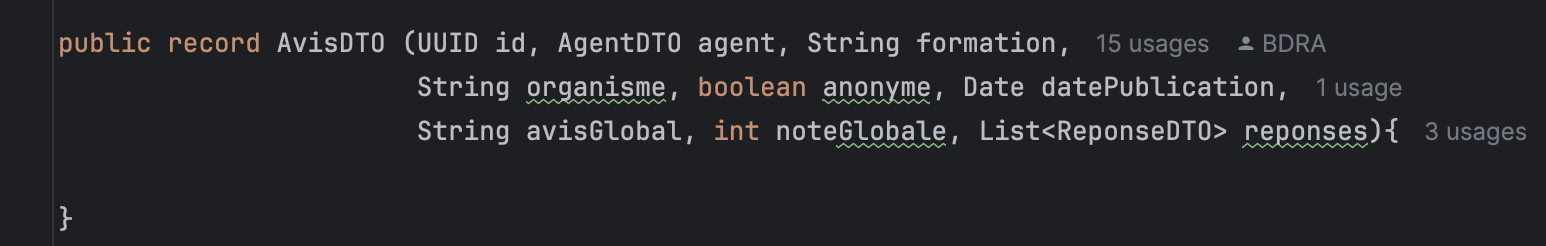
\includegraphics[width=0.8\textwidth]{images/code/AvisDTO.png}
            \caption{Exemple de classe DTO de l'application}
        \end{figure}\vspace{1cm}


        Pour nos classes Repository (DAO) nous avons utilisé Spring Data JPA pour gérer l'accès aux données. Cette classe utilise l'interface JpaRepository, pour effectuer des opérations de base telles que sauvegarder, trouver, mettre à jour et supprimer des données sans avoir à écrire beaucoup de code. 
        Cela réduit le besoin d'écrire des requêtes SQL manuellement, car Spring Data JPA génère automatiquement les requêtes nécessaires.\medskip

        \begin{figure}[h!]
            \centering
            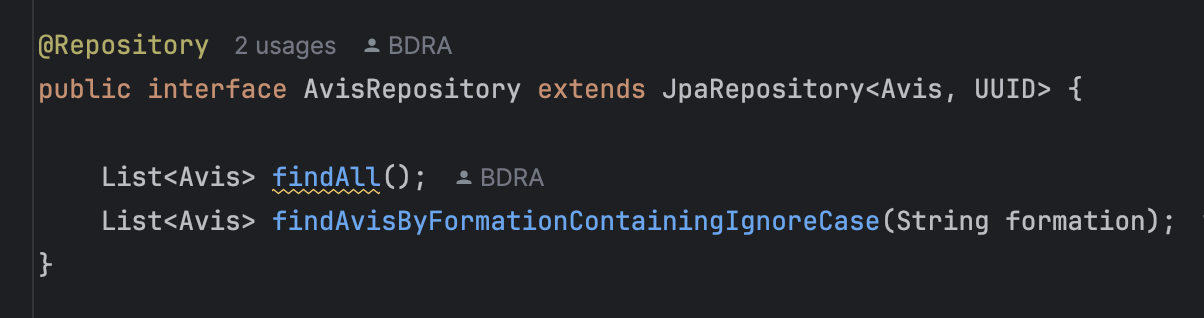
\includegraphics[width=0.8\textwidth]{images/code/DAOAvis.png}
            \caption{Exemple de classe Repository de l'application}
        \end{figure}
        \vspace{1cm}

        Les classes Services de notre application sont celles qui font appel aux DAO, dans le but de récupérer les données, les traiter et les faire transiter aux 'Controller'.
        \medskip

        \begin{figure}[h!]
            \centering
            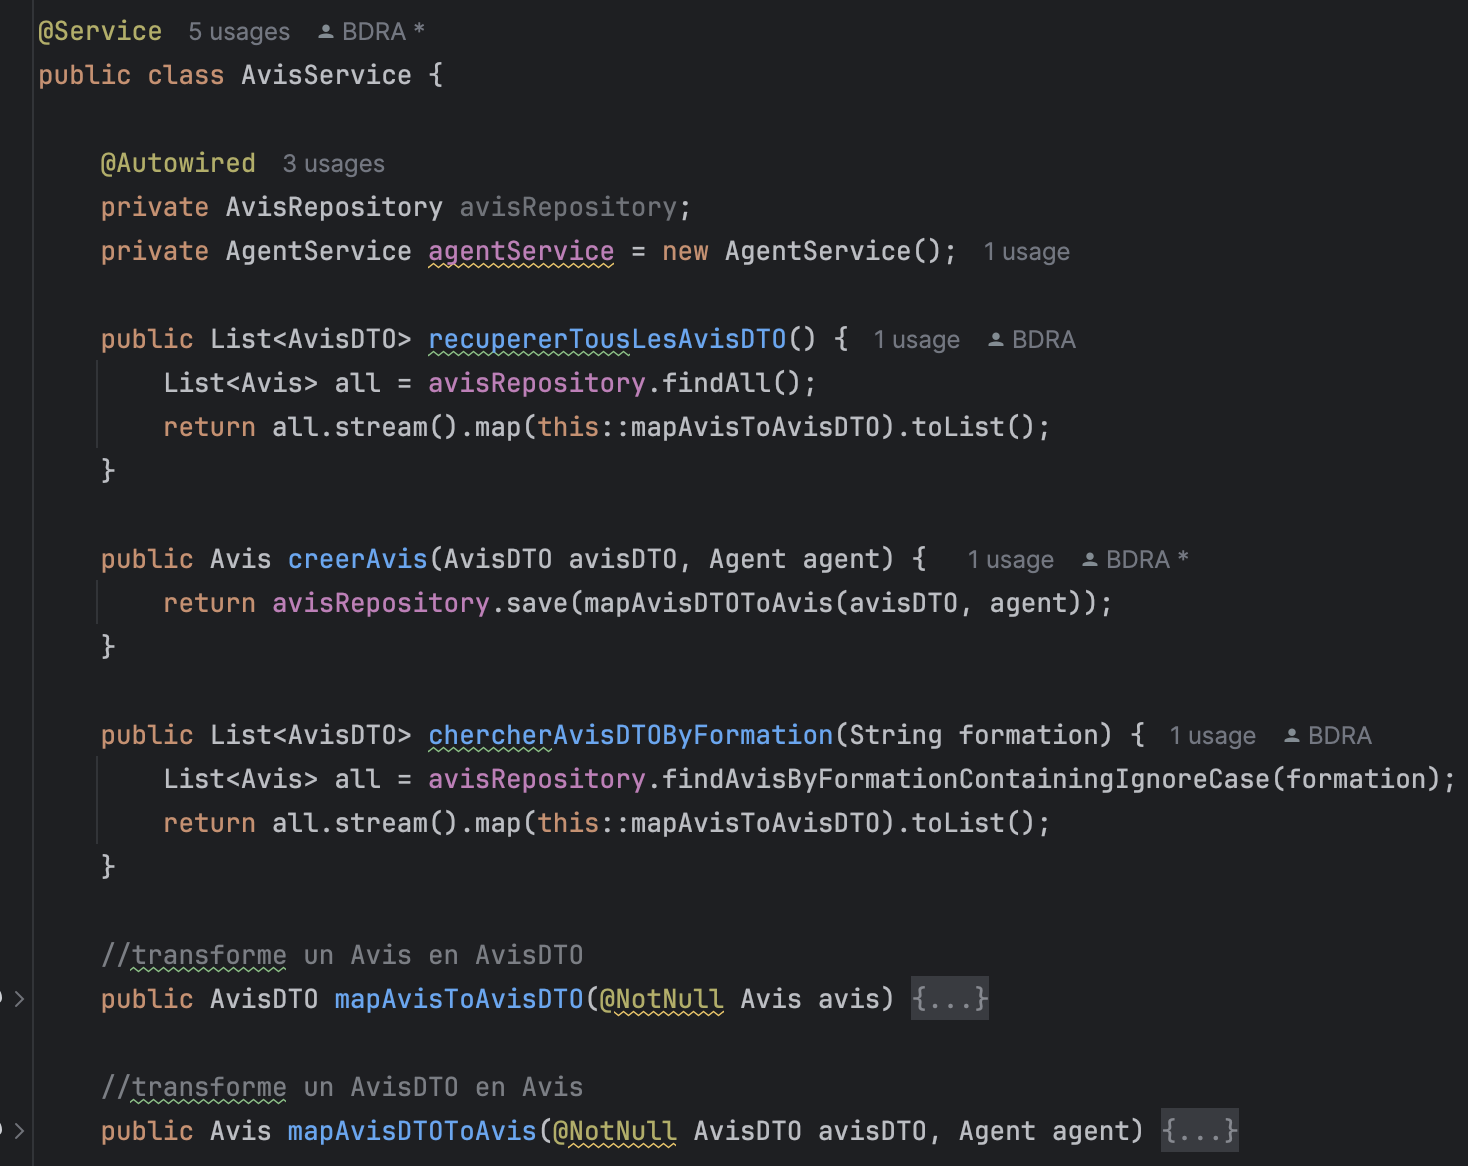
\includegraphics[width=0.8\textwidth]{images/code/avisService.png}
            \caption{Exemple de classe Service de l'application}
        \end{figure}\medskip

        Les différentes classes comportent plusieurs notations :
        \medskip

        \textbf{@Service}: permet d'indiquer que cette classe contient la logique métier et permet à Spring de détecter automatiquement cette classe.
        \medskip

        \textbf{@Autowired}: permet à Spring d'injecter une instance d'une classe existante dans la classe service. Cela permet au service d'utiliser cette instance pour accéder aux données.
        \vspace{1cm}

        Les classes Contrôleurs de notre application sont responsables de gérer les requêtes HTTP entrantes, d'appeler les services appropriés, et de renvoyer les réponses. Les contrôleurs définissent les points d'accès de l'API et orchestrent les interactions entre les utilisateurs et le système.
        \medskip

        \begin{figure}[h!]
            \centering
            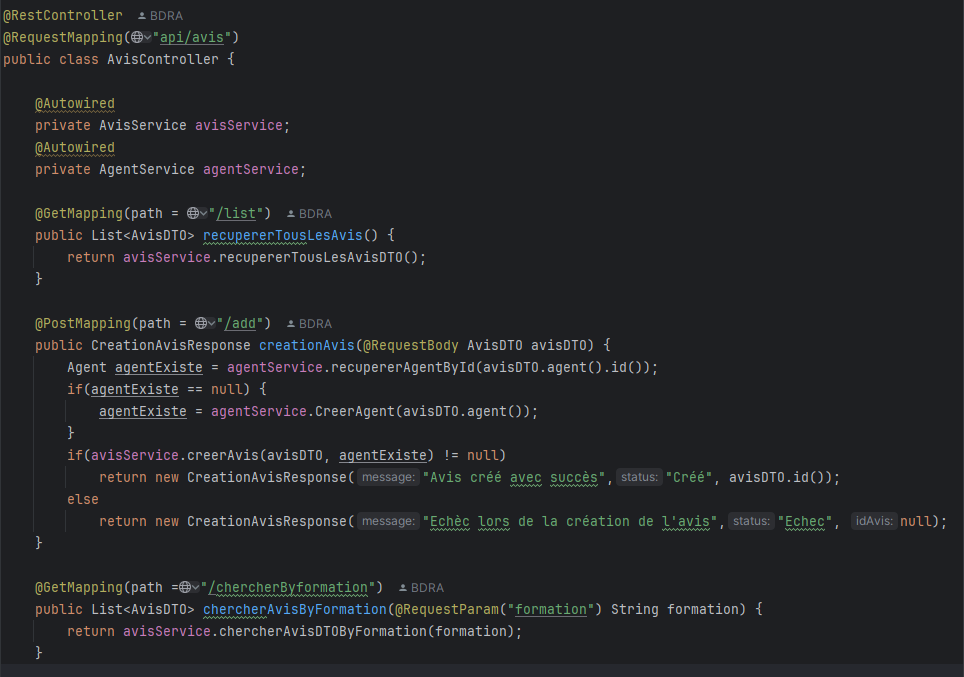
\includegraphics[width=0.8\textwidth]{images/code/controlleurAvis.PNG}
            \caption{Exemple de classe Controller de l'application}
        \end{figure}
        \medskip

        Les principales annotations utilisées dans les classes contrôleurs :
        \medskip

        \textbf{@RestController}: indique que la classe est un contrôleur ou chaque méthode de gestion de requêtes renvoie un objet directement en format JSON ou XML, plutôt que de renvoyer une vue.
        \medskip

        \textbf{@RequestMapping}: permet de mapper les requêtes HTTP à des méthodes spécifiques dans un contrôleur. Elle peut être appliqué au niveau de la classe et au niveau des méthodes pour définir des URL de base et des URL spécifiques.\\
        Dans cet exemple toutes les requêtes HTTP commençant par '/api/avis' seront dirigées vers les méthodes de ce contrôleur.
        \medskip

        \textbf{@GetMapping}: spécification de '@RequestMapping' pour les requêtes HTTP GET. Elle est utilisée pour définir les points d'accès qui répondent aux requêtes GET.
        \medskip

        \textbf{@PostMapping}: spécification de '@RequestMapping' pour les requêtes HTTP POST. Elle est utilisée pour définir les points d'accès qui répondent aux requêtes POST.
        \medskip

        

\chapter*{Bilan, conclusion et perspective}
\addcontentsline{toc}{chapter}{Bilan, conclusion et perspective}

Pour conclure, ce stage au sein de l'entreprise CNIEG a été bénifique, car il m'a permis de me familiariser avant tout avec un nouvel environnement
de développement et surtout de réaliser un produit minimun viable. Ce stage m'a permis d'apprendre un nouveau langage de programmation et d'exploiter ce que j'ai appris 
durant mon cursus universitaire.
Ça a été une opportunité de découvrir le milieu professionnel et découvrir le monde du travail au sein du département informatique.
\medskip

Notre objectif de départ qui était de consevoir un "produit minimum viable" a été atteint avec succès, 
sous la directive de mon tuteur. Toutes les problèmatiques que le tuteur m'a attibués durant le stage, 
ont été réalisées et pour chaque dificultés rencontrées j'ai pu trouvé une solution fiable.\medskip

Durant cette période, j'ai été confronté à divers défis, parmis lesquels la prise en mains du framework Angular et Spring Boot. En revenche j'ai acquis une solide compréhension de ces frameworks, en apprenant à concevoir et à développer des applications web. J'ai également amélioré mes compétences en HTML, SCSS et TypeScipt. 
\medskip

Comme toutes applications, elle reste susceptible d'avoir des mises à jour et des 
modifications.\medskip

Ce stage ma motivé à continuer de développer mes compétences en développement full stack et à explorer de nouveaux domaines, tels que l'analyse de données.
\medskip


\chapter*{Glossaire}
\addcontentsline{toc}{chapter}{Glossaire}

\begin{minipage}{\textwidth}
    \begin{minipage}{0.1\textwidth}
        \textbf{IDE}
    \end{minipage}\hfill
    \begin{minipage}{0.8\textwidth}
        Environnement de développement, un logiciel qui fournit des outils pour développer des logiciels.
    \end{minipage}
\end{minipage}

\vspace{1cm}

\begin{minipage}{\textwidth}
    \begin{minipage}{0.1\textwidth}
        \textbf{Git}
    \end{minipage}\hfill
    \begin{minipage}{0.8\textwidth}
        Logiciel de gestion de versions, qui permet de suivre les modifications de code, de gérer les branches et de collaborer avec d'autres développeurs.
    \end{minipage}
\end{minipage}

\vspace{1cm}

\begin{minipage}{\textwidth}
    \begin{minipage}{0.1\textwidth}
        \textbf{Stack}
    \end{minipage}\hfill
    \begin{minipage}{0.8\textwidth}
        Ensemble de technologies et outils utilisés pour construire une application.
    \end{minipage}
\end{minipage}

\vspace{1cm}

\begin{minipage}{\textwidth}
    \begin{minipage}{0.1\textwidth}
        \textbf{UML}
    \end{minipage}\hfill
    \begin{minipage}{0.8\textwidth}
        Unified Modeling Language, Langage de modélisation graphique et textuel pour visualiser les artefacts d’un système logiciel.
    \end{minipage}
\end{minipage}

\vspace{1cm}

\begin{minipage}{\textwidth}
    \begin{minipage}{0.1\textwidth}
        \textbf{Backlog}
    \end{minipage}\hfill
    \begin{minipage}{0.8\textwidth}
        Liste ordonnée de tâches ou de fonctionnalités à réaliser dans un projet.
    \end{minipage}
\end{minipage}

\vspace{1cm}

\begin{minipage}{\textwidth}
    \begin{minipage}{0.1\textwidth}
        \textbf{Sprint}
    \end{minipage}\hfill
    \begin{minipage}{0.8\textwidth}
        Itération de développement dans Agile, durant laquelle une équipe travaille sur des tâches spécifiques du backlog.
    \end{minipage}
\end{minipage}

\vspace{1cm}

\begin{minipage}{\textwidth}
    \begin{minipage}{0.1\textwidth}
        \textbf{API}
    \end{minipage}\hfill
    \begin{minipage}{0.8\textwidth}
        Application Programming Interface, Interface qui sert de façade pour les logiciels qui l'utilisent.
    \end{minipage}
\end{minipage}

\vspace{1cm}

\begin{minipage}{\textwidth}
    \begin{minipage}{0.1\textwidth}
        \textbf{Docker}
    \end{minipage}\hfill
    \begin{minipage}{0.8\textwidth}
        Plateforme open source automatiser le déploiement et la gestion d’applications dans des conteneurs, rendant les applications portables et cohérentes à travers différents environnements.
    \end{minipage}
\end{minipage}

\vspace{1cm}

\begin{minipage}{\textwidth}
    \begin{minipage}{0.1\textwidth}
        \textbf{NGINX}
    \end{minipage}\hfill
    \begin{minipage}{0.8\textwidth}
        Serveur web open source, léger et rapide, utilisé pour servir des sites web et gérer les connexions HTTP.
    \end{minipage}
\end{minipage}

\vspace{1cm}

\begin{minipage}{\textwidth}
    \begin{minipage}{0.1\textwidth}
        \textbf{Kubernetes}
    \end{minipage}\hfill
    \begin{minipage}{0.8\textwidth}
        Plateforme open source pour la gestion d'applications dans des conteneurs, permettant de déployer des services.
    \end{minipage}
\end{minipage}

\vspace{1cm}

\begin{minipage}{\textwidth}
    \begin{minipage}{0.1\textwidth}
        \textbf{Mapper}
    \end{minipage}\hfill
    \begin{minipage}{0.8\textwidth}
        Mettre en correspondance les champs de plusieurs bases dedonnées
    \end{minipage}
\end{minipage}

\vspace{1cm}

\begin{minipage}{\textwidth}
    \begin{minipage}{0.1\textwidth}
        \textbf{URL}
    \end{minipage}\hfill
    \begin{minipage}{0.8\textwidth}
        Uniform Resource Locator, identifie de manière unique une ressource sur Internet.
    \end{minipage}
\end{minipage}

\vspace{1cm}

\begin{minipage}{\textwidth}
    \begin{minipage}{0.1\textwidth}
        \textbf{Framework}
    \end{minipage}\hfill
    \begin{minipage}{0.8\textwidth}
        Ensemble de composants logiciels structurels pour développer des logiciels. 
    \end{minipage}
\end{minipage}

\vspace{1cm}

\begin{minipage}{\textwidth}
    \begin{minipage}{0.1\textwidth}
        \textbf{JSON}
    \end{minipage}\hfill
    \begin{minipage}{0.8\textwidth}
        Java Script Object Notation, format de texte utilisé pour représenter les données structurées basées sur la syntaxe des objets JavaScript.
    \end{minipage}
\end{minipage}

\vspace{1cm}

\begin{minipage}{\textwidth}
    \begin{minipage}{0.1\textwidth}
        \textbf{JPA}
    \end{minipage}\hfill
    \begin{minipage}{0.8\textwidth}
        Java Persistence API, spécification Java pour gérer les données relationnelles via le mapping objet-relationnel (ORM). Facilite l’interaction entre les objets Java et les bases de données.
    \end{minipage}
\end{minipage}

\vspace{1cm}

\begin{minipage}{\textwidth}
    \begin{minipage}{0.1\textwidth}
        \textbf{CRUD}
    \end{minipage}\hfill
    \begin{minipage}{0.8\textwidth}
        Create Read Upadate Delete, acronyme qui désigne les qu’âtres opérations de base utilisées dans la gestion des données persistantes.    
    \end{minipage}
\end{minipage}

\vspace{1cm}

\begin{minipage}{\textwidth}
    \begin{minipage}{0.1\textwidth}
        \textbf{ORM}
    \end{minipage}\hfill
    \begin{minipage}{0.8\textwidth}
        Object Relational Mapping, technique permettant de convertir les données entre les systèmes de type objet et les bases de données relationnelles. Hibernate est un exemple populaire d’ORM.    
    \end{minipage}
\end{minipage}

\vspace{1cm}

\begin{minipage}{\textwidth}
    \begin{minipage}{0.1\textwidth}
        \textbf{DTO}
    \end{minipage}\hfill
    \begin{minipage}{0.8\textwidth}
        Data Transfer Object, Objet utilisé pour transférer des données entre différentes couches d’une application.
    \end{minipage}
\end{minipage}

\vspace{1cm}

\begin{minipage}{\textwidth}
    \begin{minipage}{0.1\textwidth}
        \textbf{DAO}
    \end{minipage}\hfill
    \begin{minipage}{0.8\textwidth}
        Data Access Object, Modèle de conception fournissant une abstraction pour les opérations CRUD sur les entités.    
    \end{minipage}
\end{minipage}

\vspace{1cm}

\begin{minipage}{\textwidth}
    \begin{minipage}{0.1\textwidth}
        \textbf{HTTP}
    \end{minipage}\hfill
    \begin{minipage}{0.8\textwidth}
        Hypertext Transfer Protocol, est un protocole de transfert de données dans le web. 
    \end{minipage}
\end{minipage}

\vspace{1cm}

\begin{minipage}{\textwidth}
    \begin{minipage}{0.1\textwidth}
        \textbf{GET}
    \end{minipage}\hfill
    \begin{minipage}{0.8\textwidth}
        Méthode HTTP qui demande des données à partir d'un serveur.
    \end{minipage}
\end{minipage}

\vspace{1cm}

\begin{minipage}{\textwidth}
    \begin{minipage}{0.1\textwidth}
        \textbf{POST}
    \end{minipage}\hfill
    \begin{minipage}{0.8\textwidth}
        Méthode HTTP qui envoie les données au serveur.
    \end{minipage}
\end{minipage}


\addcontentsline{toc}{chapter}{Table des figures}
\listoffigures

\nocite{*}

\addcontentsline{toc}{chapter}{Bibliographie}

\printbibliography


\chapter*{Annexes}
\addcontentsline{toc}{chapter}{Annexes}
 
\section*{Page d'accueil}
Dans notre site nous avons un seul utilisateur qui est l'agent. Au lancement du site la page principale s'affichera avec la liste des avis avec les fonctionnalités du site.
\medskip

\begin{figure}[h!]
    \centering
    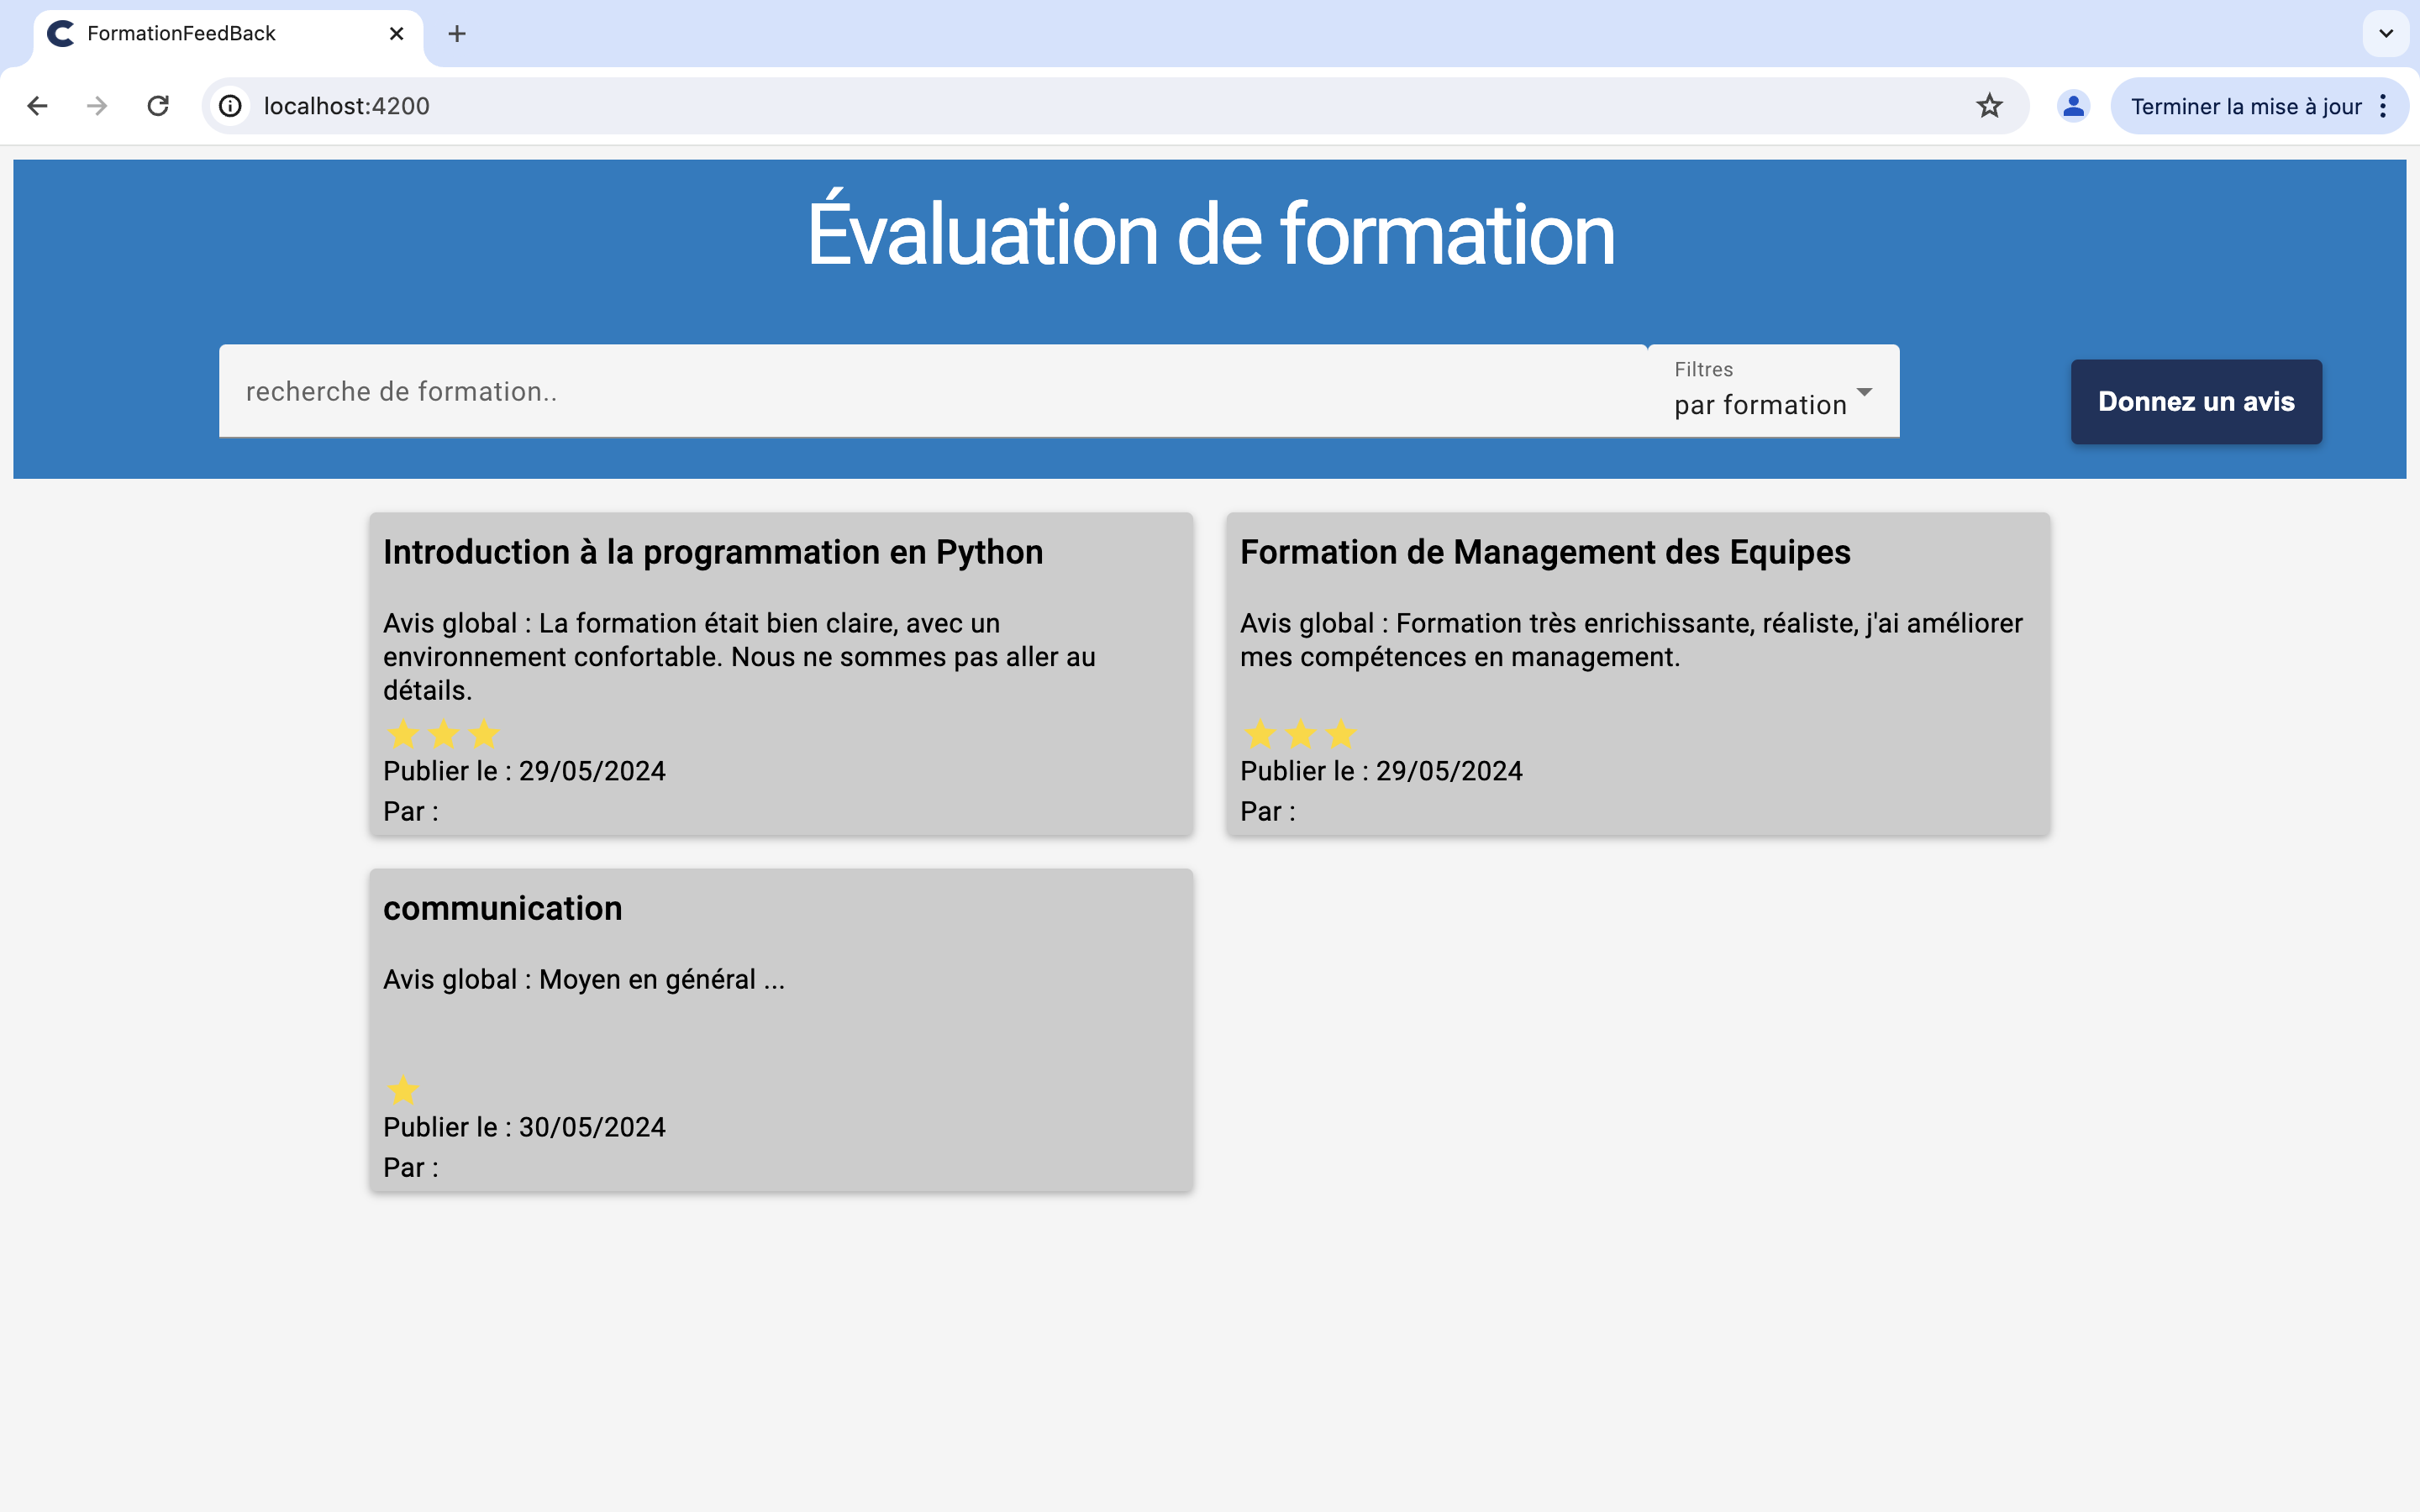
\includegraphics[width=1\textwidth]{images/fenetres/accueil.png}
    \caption{Page Principale}
\end{figure}

\newpage

\section*{Ajouter un avis}
Lorsque l'agents veut ajouter un avis sur une formation qu'il à suivi, il clique sur le bouton 'Donnez un avis', une fenêtre modale du formulaire s'ouvre, il remplit les champs nécessaires. 
\medskip

\begin{figure}[h!]
    \centering
    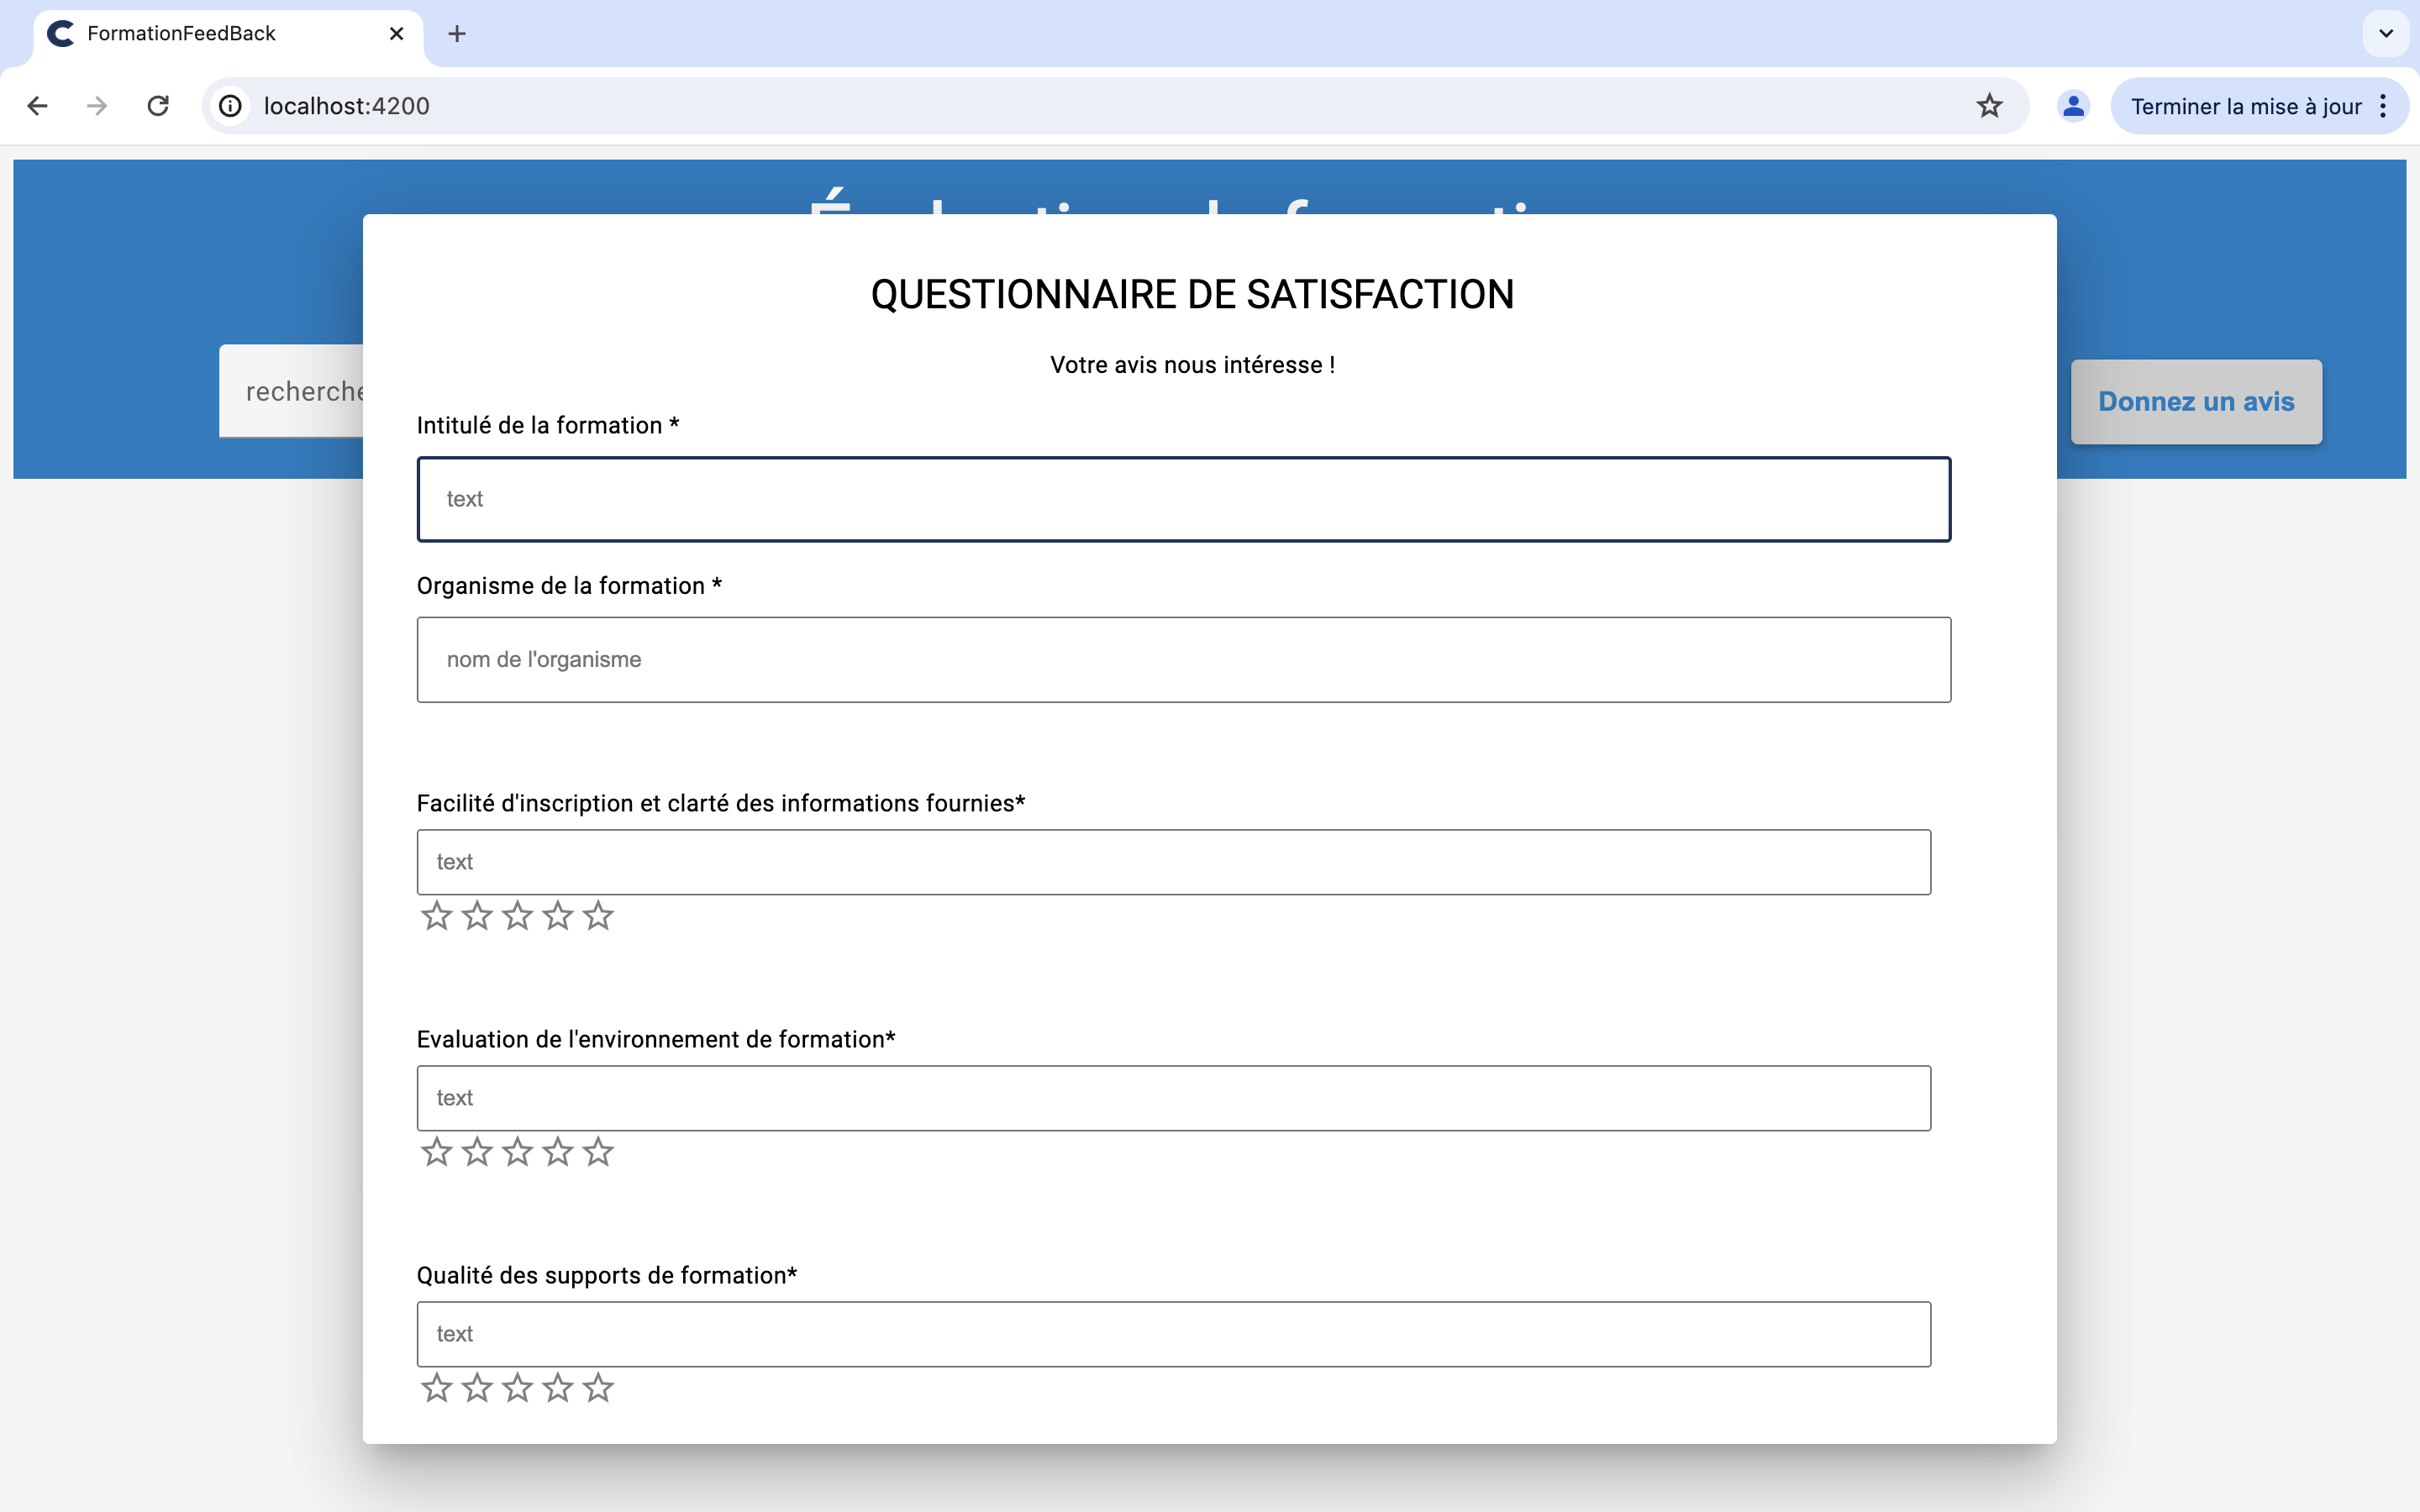
\includegraphics[width=1\textwidth]{images/fenetres/AjouterAvis.png}
    \caption{Formulaire d'ajout d'un avis}
\end{figure}

\newpage

\section*{Rechercher un avis}
On peut aussi rechercher un avis par des filtres, exemple mot clé où par formation les mieux notée.
\medskip

\begin{figure}[h!]
    \centering
    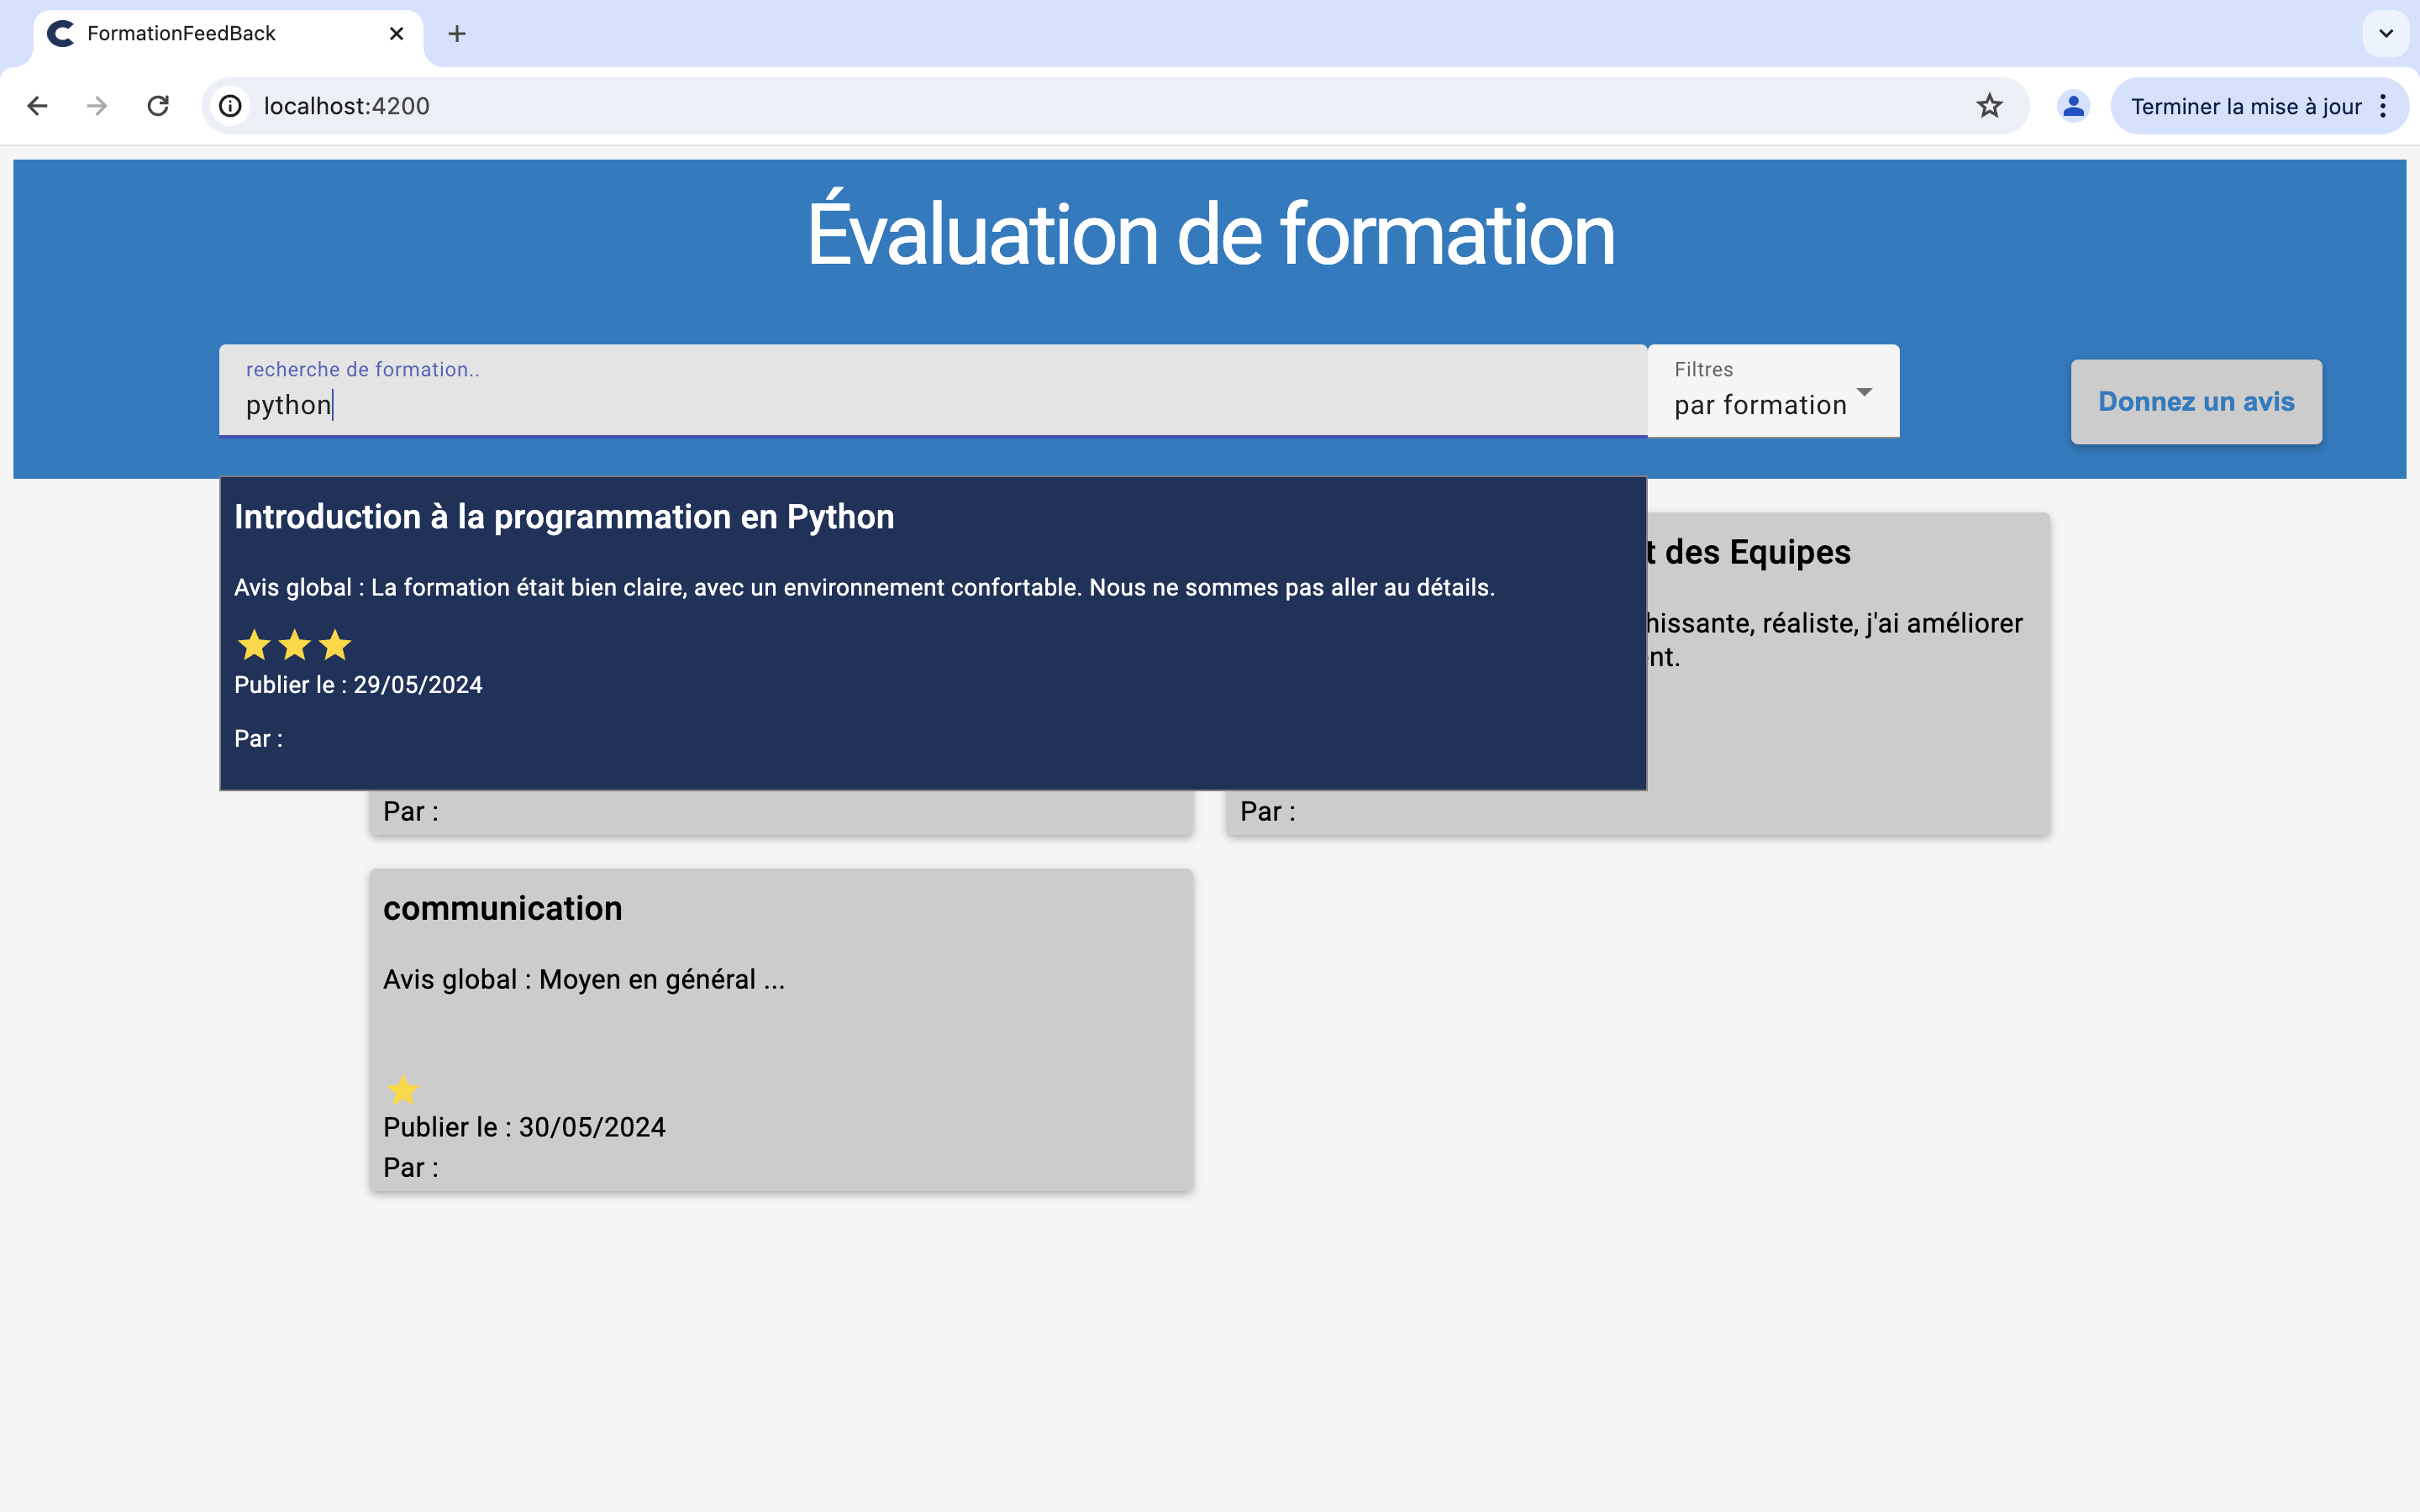
\includegraphics[width=1\textwidth]{images/fenetres/rechercheAvis.png}
    \caption{Rechercher un avis avec un mot clé}
\end{figure}

\newpage

\section*{Détails d'un avis}
L'agent peut consulter le détails d'un avis qu'il sélectionne.
\medskip

\begin{figure}[h!]
    \centering
    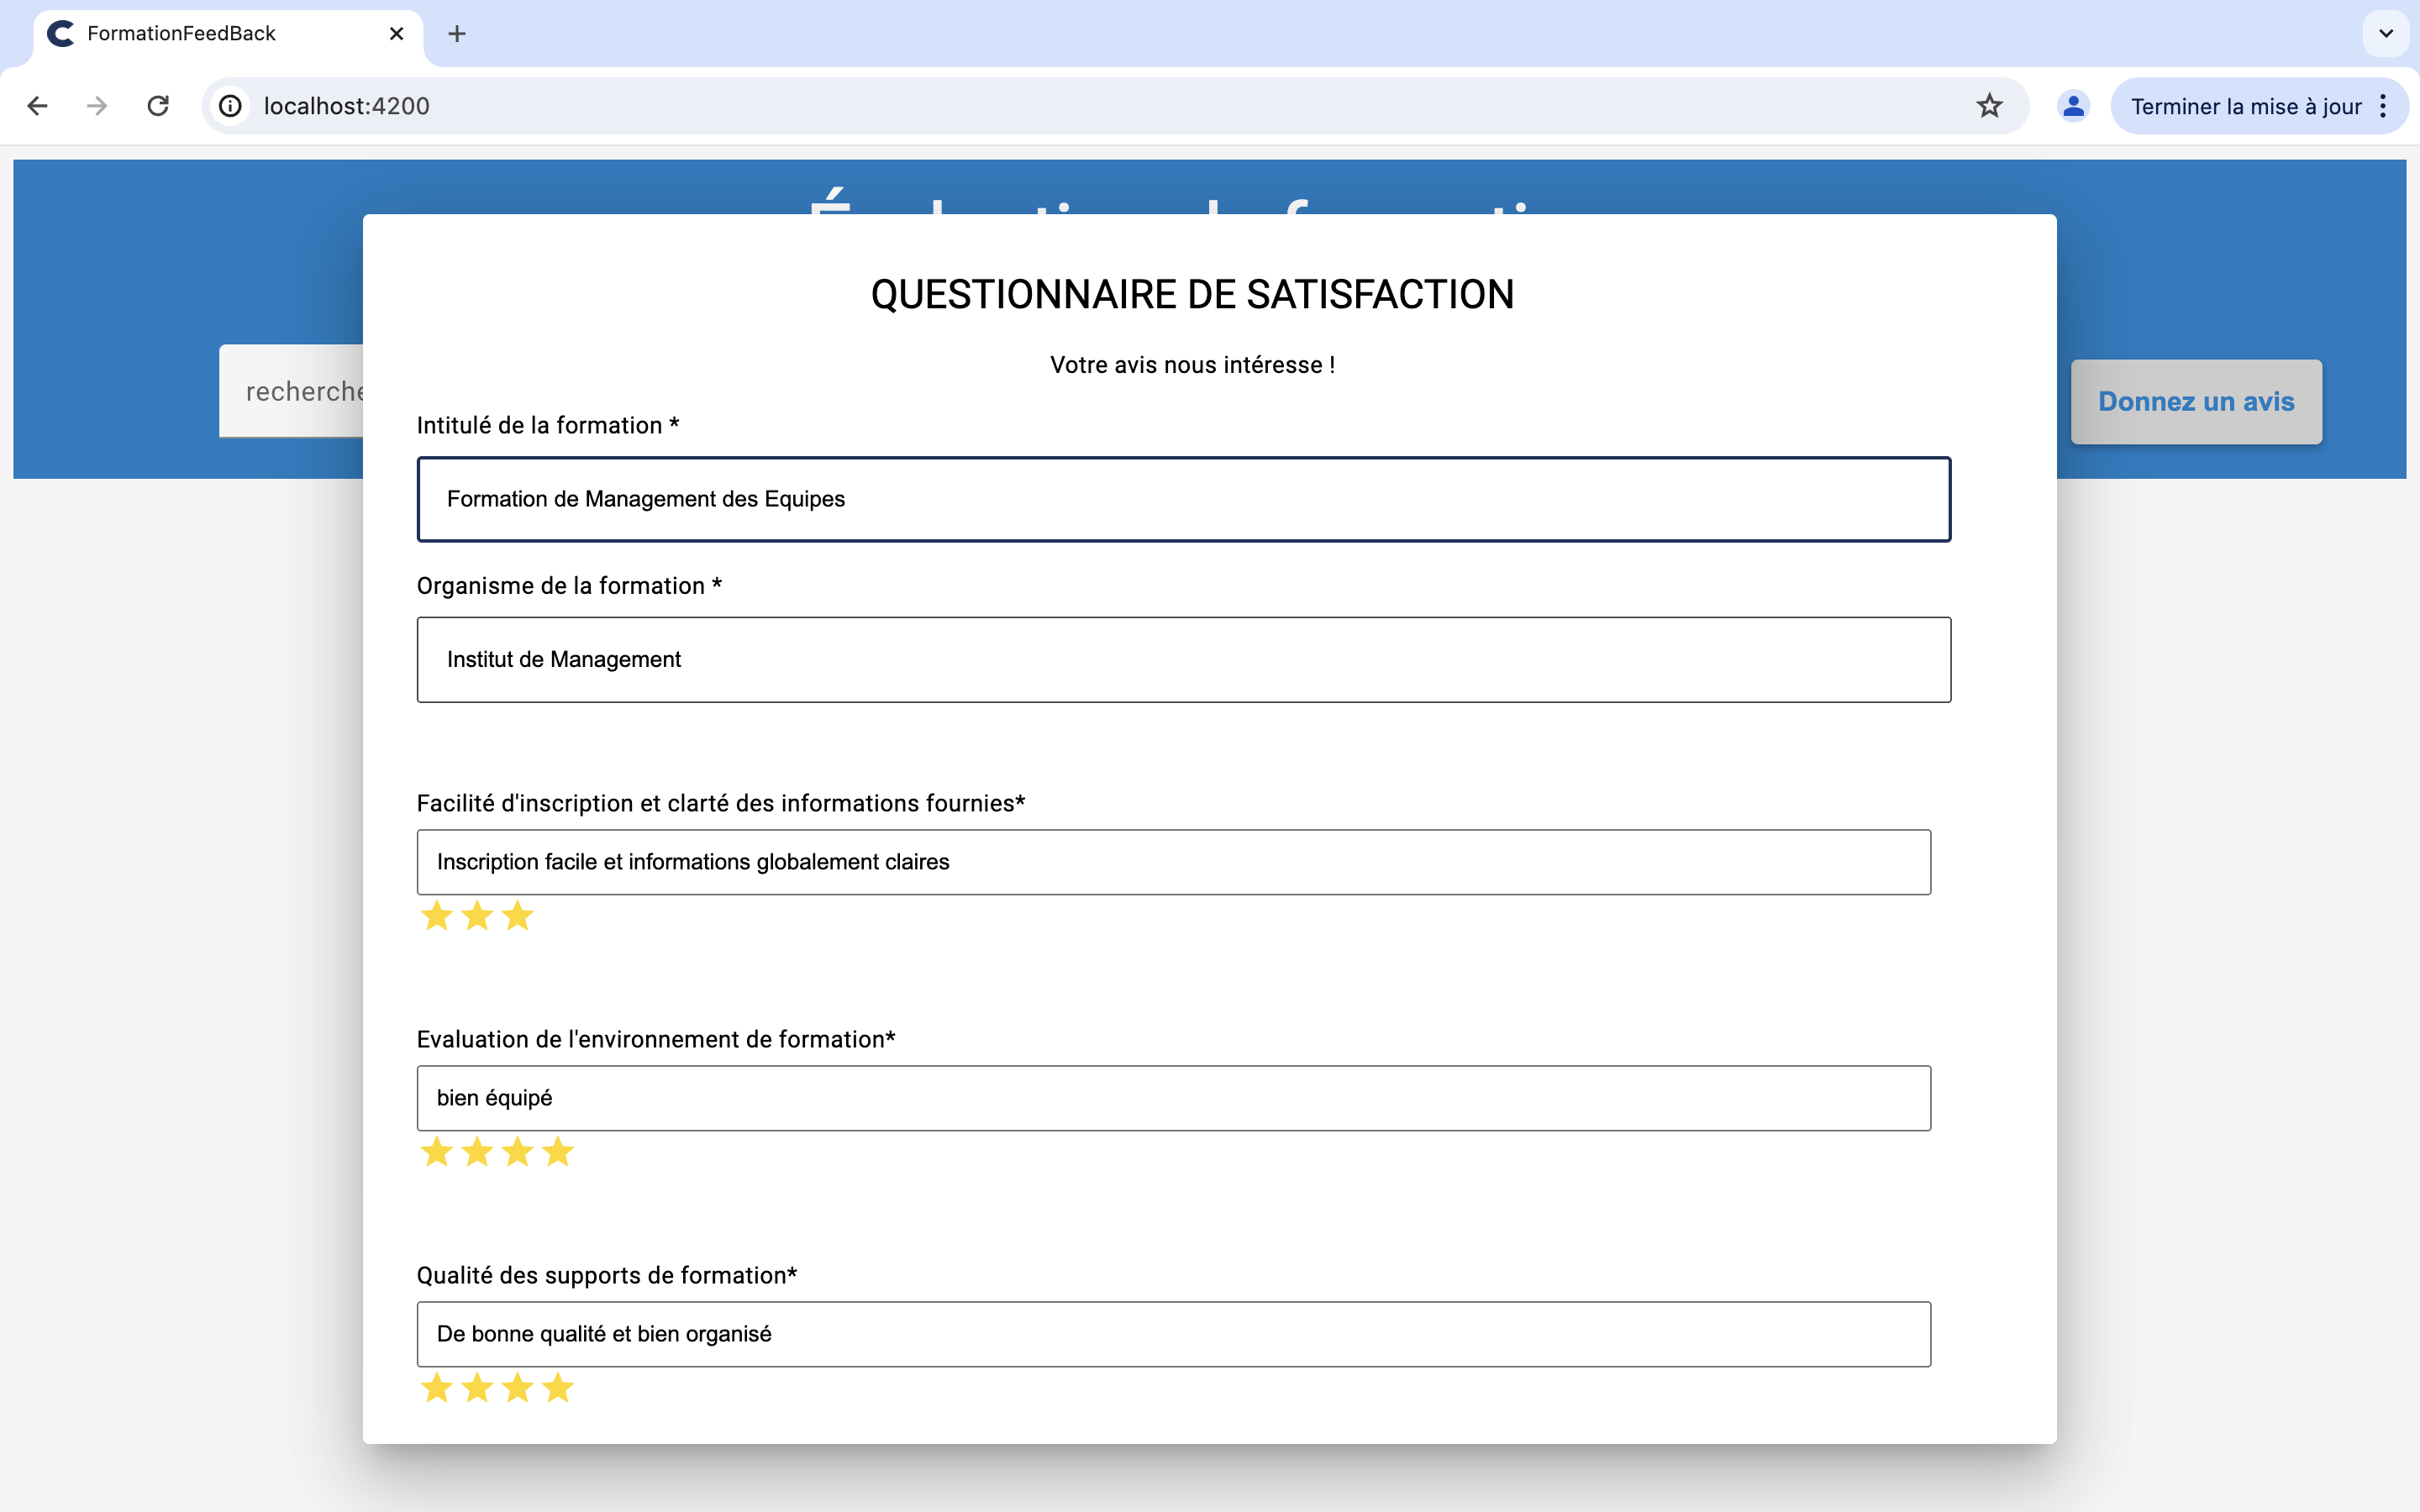
\includegraphics[width=1\textwidth]{images/fenetres/DetailsAvis.png}
    \caption{Détails d'un avis}
\end{figure}
\medskip


% ...

\end{document}